\documentclass[11pt]{article}

\usepackage[margin=1in]{geometry}
\usepackage{graphicx}
\usepackage{booktabs}
\usepackage{amsmath}
\usepackage{amssymb}
\newcommand{\ind}{\mathbf{1}}  % indicator function
\usepackage[hidelinks]{hyperref}
\usepackage{natbib}
\usepackage{caption}
\usepackage{float}

\graphicspath{{../figures/}}

% Auto-generated numeric facts (written by 3a and 3b). Re-running those
% notebooks refreshes every number below, so the paper cannot silently
% drift out of sync with the code.
% AUTO-GENERATED by 3a_supervised_learning.ipynb -- do not edit by hand.
\newcommand{\NRows}{13,325}
\newcommand{\NFeatures}{16}
\newcommand{\NTrain}{10,719}
\newcommand{\NTest}{2,606}
\newcommand{\CutoffDate}{2025-04-15}
\newcommand{\BestClf}{Random Forest}
\newcommand{\BestReg}{Random Forest}

% AUTO-GENERATED by 3b_unsupervised_clustering.ipynb -- do not edit by hand.
\newcommand{\BestK}{2}
\newcommand{\Silhouette}{0.531}
\newcommand{\NPairs}{349}
\newcommand{\AriAgglo}{0.951}
\newcommand{\AriGmm}{0.329}


\title{Predicting and Clustering Retail Food Prices in Rwanda:\\
A Comparison of Statistical, Ensemble, and Neural Approaches\\
Using Market, Climate, and Macroeconomic Data}
\author{Ahourdet Donambi Thierry 101201 \\ MSc Big Data Analytics, Adventist University of Central Africa \\ MSDA 9213: Data Mining}
\date{September 2026}

\begin{document}

\maketitle

\begin{abstract}
Food price volatility is a persistent policy concern in East Africa, yet predictive analyses are often constrained by data that is slow or restricted
to access. This study builds a complete data mining pipeline on four freely available open datasets: World Food Programme retail food price records for
Rwanda (2020--2026), NASA POWER climate data (temperature, precipitation, soil moisture), the USD/RWF exchange rate, and Rwanda's Consumer Price Index. We
classify whether a commodity's price rises month-over-month, regress the price level, and cluster market--commodity pairs by price and climate profile. Four
algorithms per supervised task  logistic/linear regression, random forest, gradient boosting, and a multi-layer perceptron  are compared on a
chronological split. Three data-leakage defects were identified and corrected, one arising from the publication lag of official CPI statistics. Price level
appeared highly predictable (random forest, $R^2 = 0.94$), but a naive persistence benchmark achieved lower error than every trained model (RMSE 295
versus 466 RWF), showing the fit reflects autocorrelation rather than forecasting skill. Price direction, admitting no such trivial rule, remained
genuinely difficult (best ROC-AUC 0.641), though tuning improved it and a controlled ablation showed that enriching the features beyond temperature
raised ROC-AUC for every model family  a gain attributable chiefly to precipitation rather than the macroeconomic series added for that purpose.
Clustering isolated Rwanda's cooler, wetter Northern Province. We conclude that level and direction are qualitatively different problems and that
level-prediction results must be reported against a persistence benchmark.
\end{abstract}

\section{Introduction}

Retail food prices in East Africa are shaped by local agricultural conditions, transport costs, seasonal harvest cycles, and broader
macroeconomic pressures. Rwanda has pronounced regional climate variation from the cooler volcanic highlands of the Northern Province to the
warmer lowlands elsewhere  that plausibly affects the price and availability of weather-sensitive crops. Predicting food price movements,
and identifying markets that behave similarly, has direct relevance for food security monitoring and early-warning systems.

This project was deliberately scoped around \textbf{freely and immediately accessible} open data rather than sources requiring registration or approval
(such as Demographic and Health Survey microdata), given the constrained timeline of this assignment. The specific objectives are to:

\begin{enumerate}
  \item Determine whether a commodity's retail price at a given market is likely to \emph{increase} from one month to the next (classification);
  \item Predict the retail price \emph{level} itself (regression);
  \item Identify natural groupings of markets and commodities based on shared price and climate characteristics (clustering);
  \item Apply and evaluate a model-improvement step (hyperparameter tuning), reporting honestly whether it helped.
\end{enumerate}

Two themes run through the paper. The first is the deliberate identification and correction of data leakage: panel-structured price data over time is
unusually susceptible to look-ahead bias, and we document three separate defects of this kind, each caught and corrected rather than left in place.
The second is a willingness to report results that contradict the hypothesis that motivated collecting the data  specifically, that the macroeconomic
features added to improve directional prediction appear to contribute less than the climate features added alongside them.

All Jupyter notebooks, data, and figures are available at \url{https://github.com/Elthiero/auca_data_mining/tree/main/mid_exam}.


\section{Methods}

\subsection{Data Sources and Description}
\label{sec:data}

Four open datasets were combined:

\begin{itemize}
  \item \textbf{WFP Food Prices} \citep{wfp_food_prices}: monthly retail and wholesale commodity price records, extracted from the global WFP file by streaming SQL query. After filtering to kilogram-denominated units, retail price type, and records flagged \texttt{actual} (excluding estimated or imputed source values), the data covers 5 provinces, 33 markets, and 14 commodity groups.
  \item \textbf{NASA POWER} \citep{nasa_power}: daily temperature (T2M), precipitation (PRECTOTCORR), and profile soil moisture (GWETPROF) at each province's approximate centroid. Precipitation and soil moisture were added to capture agronomic conditions more directly than air temperature, since crop yield responds more immediately to rainfall and soil water availability.
  \item \textbf{USD/RWF exchange rate} \citep{yahoo_finance_fx}: monthly average closing rate, a proxy for imported-commodity cost pressure.
  \item \textbf{Rwanda Consumer Price Index} \citep{nisr_cpi}: general and food-specific CPI, a proxy for broad inflationary pressure.
\end{itemize}

WFP prices and NASA POWER data were merged on (\texttt{date}, \texttt{province}), with climate features engineered on an isolated per-province timeline before being joined back  avoiding the duplication that would result from computing lags directly on the many-rows-per-date
price table. Engineered features include, for temperature and precipitation, a monthly anomaly relative to the climatological mean, one- to three-month
lags, and a three-month rolling average; soil moisture, already a smoothed measure, receives a single one-month lag. Exchange rate and CPI are
national-level series and were merged on \texttt{date} alone.

The final modelling dataset contains \NRows{} observations.

\subsection{Data Cleaning and Leakage Correction}
\label{sec:leakage}

Three data-integrity defects were identified during development. We describe them explicitly because each represents a distinct mechanism by which
future information can reach a model, and because the third arises from a property of official statistics that is easy to overlook.

\paragraph{(1) Backward-filled lag features:} An initial implementation filled missing lagged climate and price features with
\texttt{ffill().bfill()}. The \texttt{bfill} step copies a \emph{future} observation backward into an earlier row that has no history yet 
information unavailable at prediction time in any real deployment. The fix uses \texttt{ffill} only and explicitly drops rows that still lack genuine
history, rather than fabricating values for them.

\paragraph{(2) Label computed against an inconsistent feature:} The classification target \texttt{price\_direction} was originally computed before \texttt{price\_prev\_month} was finalised, and the grouping key used to construct the lag (\texttt{commodity\_group}) differed from the key later
used to fill it (\texttt{commodity\_name}). The stored label could therefore disagree with the feature it was nominally derived from. The corrected
pipeline uses a single consistent key  (\texttt{province}, \texttt{market\_name}, \texttt{commodity\_name})  throughout, and computes
the target only after the lag feature is final.

\paragraph{(3) CPI publication lag:} Unlike exchange rates, which are observed in real time, national statistical offices publish a given month's
CPI several weeks into the \emph{following} month. Merging a price row against the same-month CPI value would supply a figure that had not yet been
released  the same class of defect as (1), reaching the model through a new source. We therefore shift each CPI observation's availability date
forward by one month before merging, so a price row dated month $M$ sees only the index reported for month $M-1$. We do not have NISR's exact release
calendar, so the one-month lag is a conservative, explicitly disclosed assumption rather than a verified fact.

\paragraph{A data-cost decision:} The cleaning notebook prints the row cost of each macroeconomic column before dropping anything. That diagnostic showed a stark asymmetry: six of the seven
columns cost zero rows, while year-over-year CPI change alone would have deleted 2{,}025 rows (15.2\%)  necessarily the earliest year of the series,
since a year-over-year change is undefined until twelve months of history exist, and therefore precisely the rows a chronological split depends on for
training. That is a steep price for a single feature largely redundant with month-over-month inflation. We instead drop that
\emph{column} and retain the \emph{rows}. The choice is recorded in the cleaning notebook as a reversible flag, alongside a printed table of the row
cost each macroeconomic column would impose, so the trade-off is made deliberately rather than by accident.

\subsection{Exploratory Data Analysis}

Exploratory analysis established several facts that directly shaped the modelling choices:

\begin{itemize}
  \item \texttt{price\_rwf} is heavily right-skewed (skewness $\approx 2.65$), motivating a $\log(1+x)$ transform for regression, with predictions back-transformed via \texttt{expm1} for reporting in RWF (Figure~\ref{fig:price_dist}).
  \item Price level differs by an order of magnitude across commodity groups (Figure~\ref{fig:price_commodity}), so outlier screening is performed within commodity groups rather than globally.
  \item The classification target is moderately imbalanced ($\approx 60/40$), motivating evaluation by precision, recall, F1, and ROC-AUC rather than accuracy alone (Figure~\ref{fig:class_balance}).
  \item Northern Province is roughly $3^{\circ}$C cooler than the rest of the country (Figure~\ref{fig:temp_province}), consistent with its volcanic highland geography.
  \item Market coverage is uneven, with Eastern and Southern Provinces contributing the large majority of observations (Figure~\ref{fig:obs_province}).
  \item Temperature correlates only weakly with price in aggregate (Figure~\ref{fig:corr_heatmap}), though more strongly for weather-sensitive commodities than for processed staples (Figure~\ref{fig:temp_scatter}).
\end{itemize}

\paragraph{Testing the enrichment directly.} Because precipitation, soil moisture, exchange rate, and CPI were added specifically to improve
directional prediction, we tested whether they in fact differ between rising and falling-price observations rather than assuming they would. Among the
added predictors, precipitation shows by far the largest separation between the classes (3.01\,mm versus 3.33\,mm mean daily rainfall), while the
month-over-month macroeconomic changes differ by less than 0.007 in every case. Provincial climate profiles also show that Northern Province is not only the coolest province ($17.5^{\circ}$C) but by a wide margin the wettest (4.52\,mm/day against 1.12--3.23\,mm elsewhere). Both findings anticipate the interpretation in Section~\ref{sec:ablation}.

\begin{figure}[H]
  \centering
  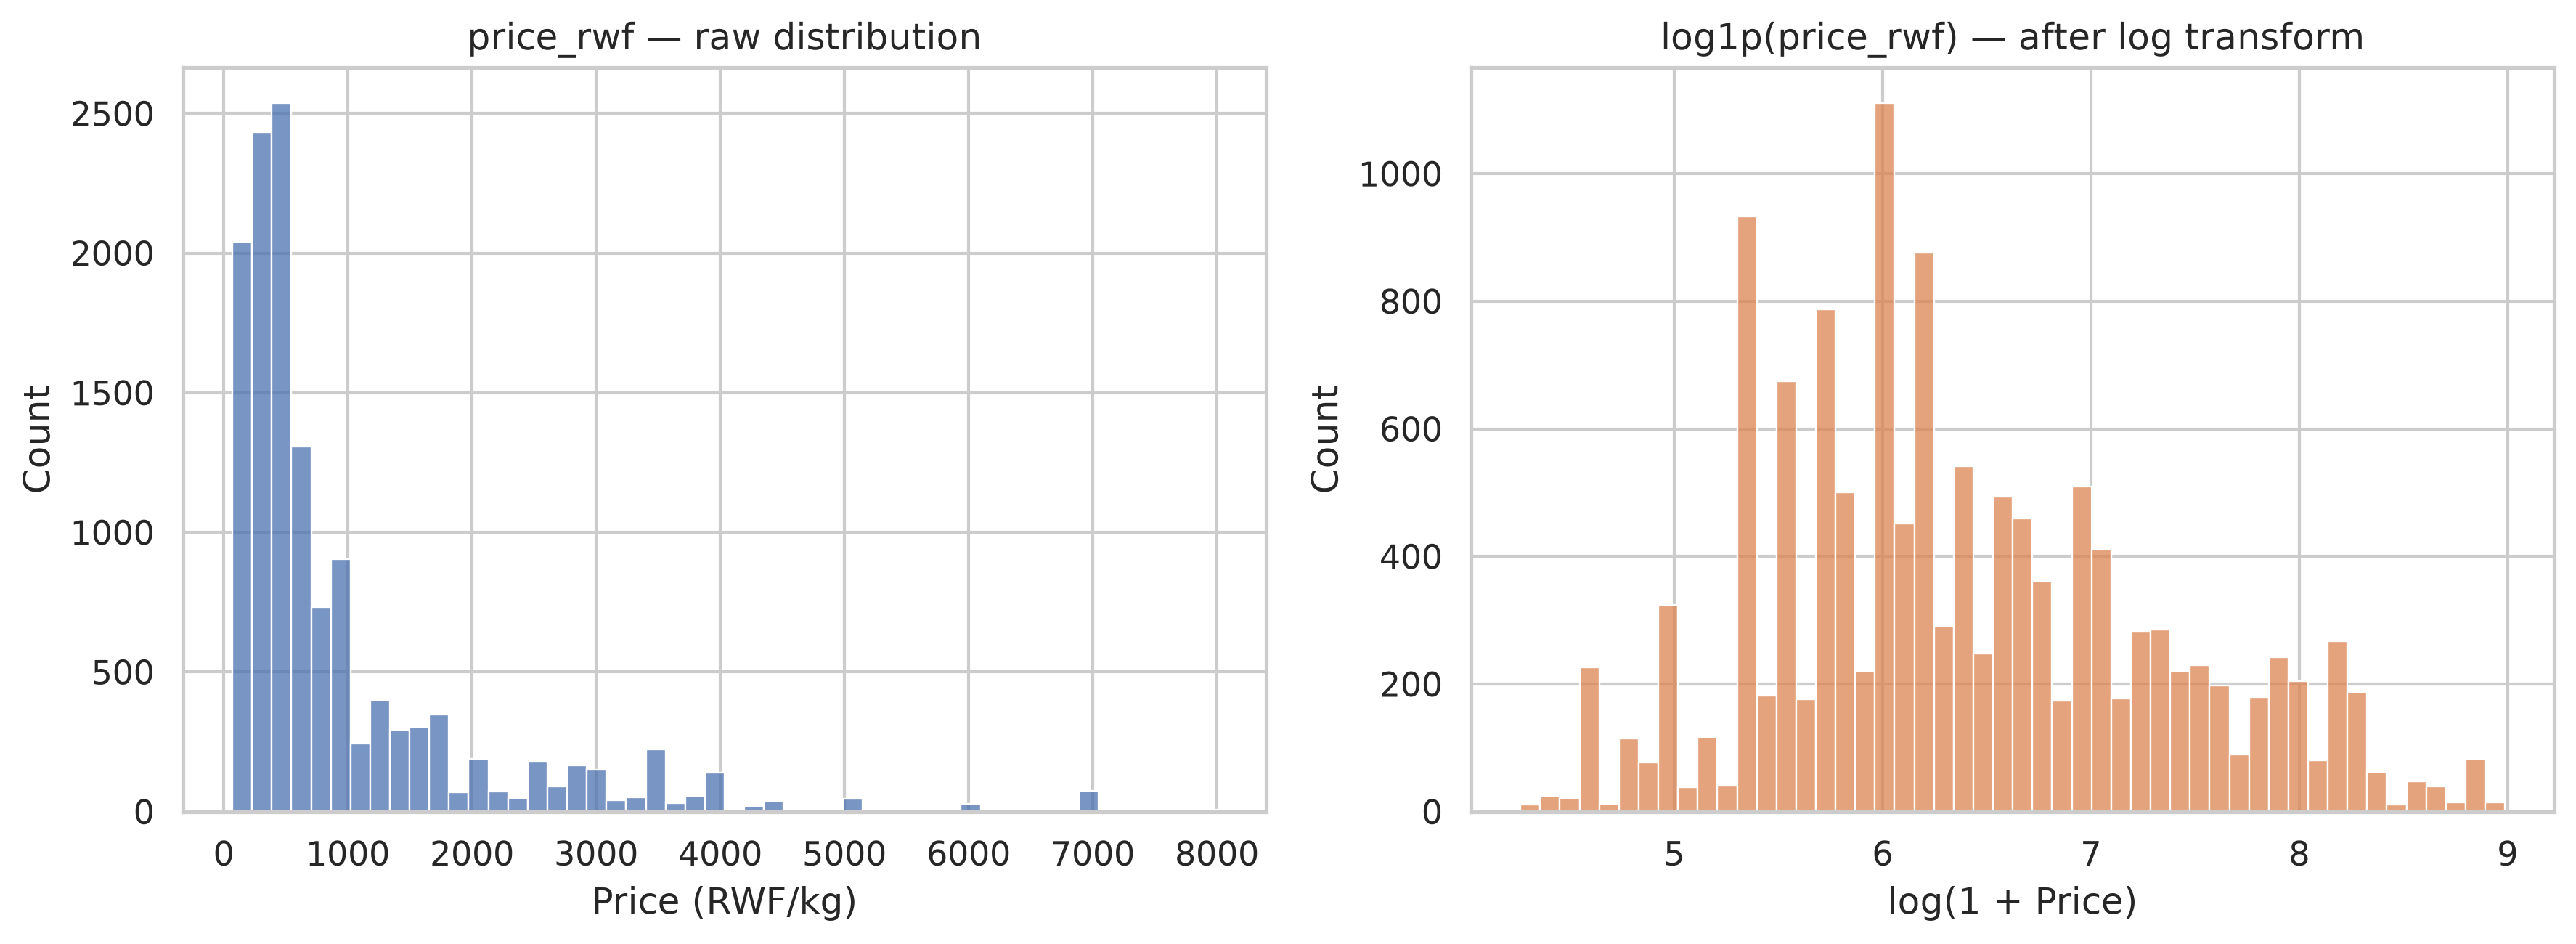
\includegraphics[width=0.85\textwidth]{price_distribution_raw_vs_log}
  \caption{Distribution of \texttt{price\_rwf}, raw and log-transformed.}
  \label{fig:price_dist}
\end{figure}

\begin{figure}[H]
  \centering
  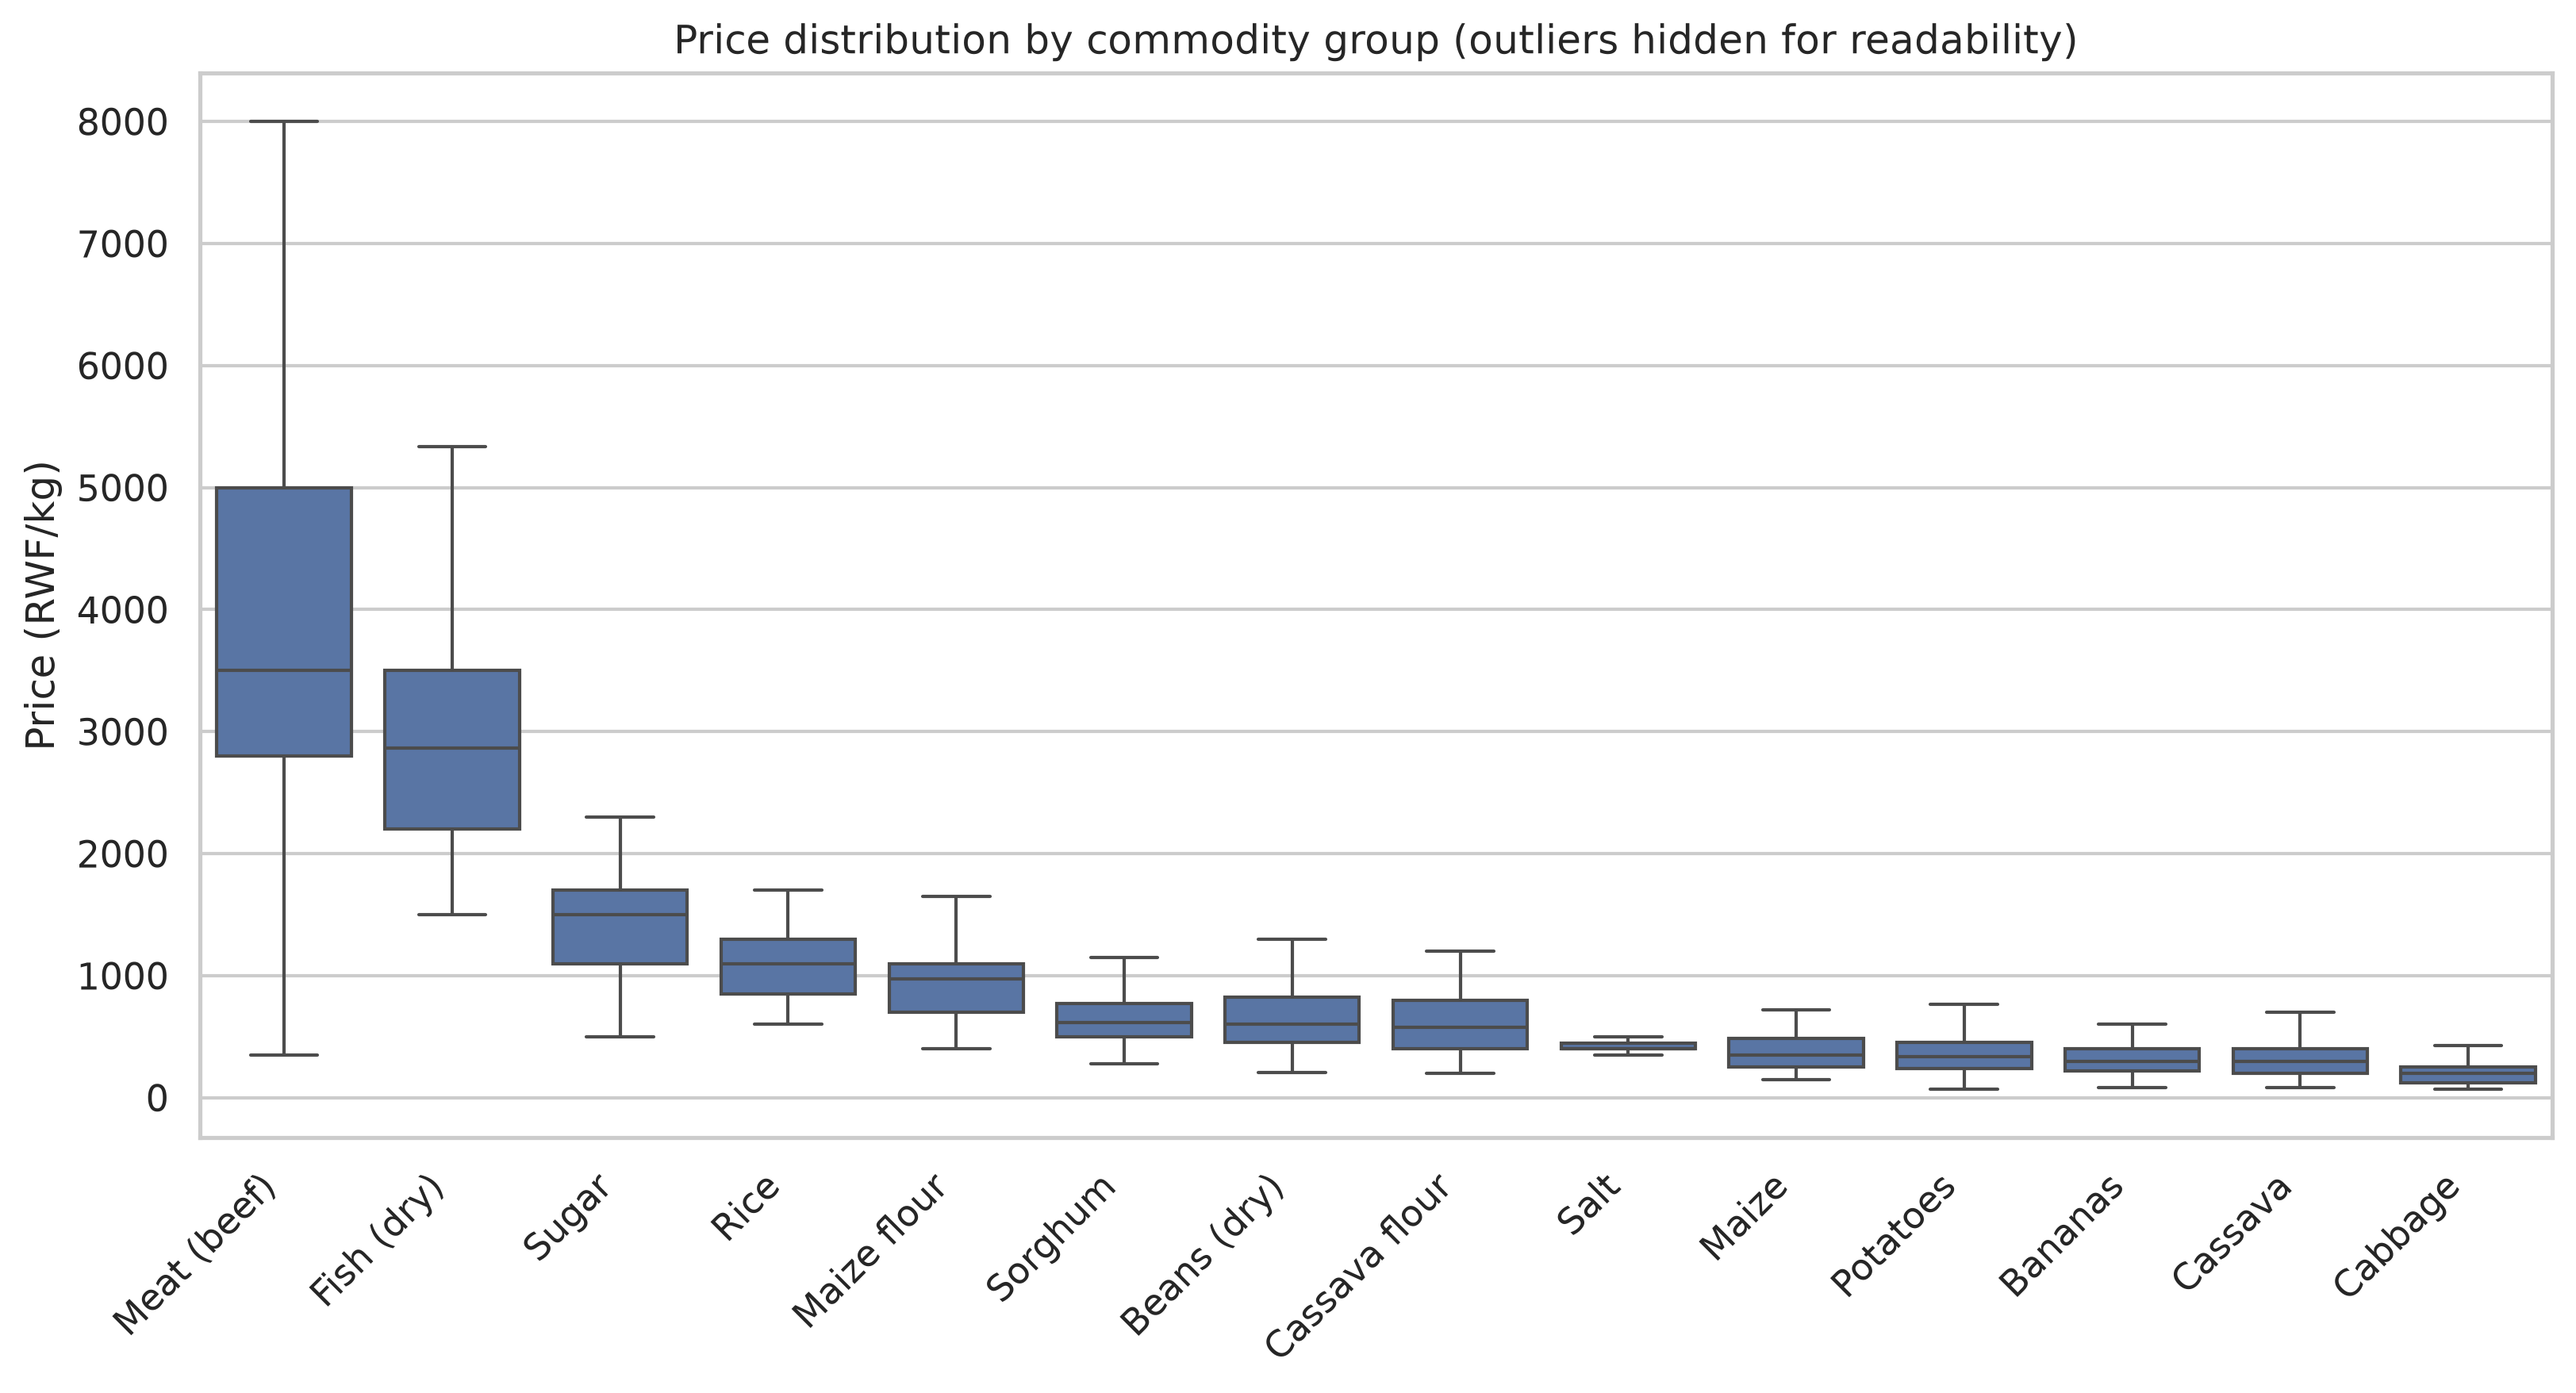
\includegraphics[width=0.85\textwidth]{price_by_commodity_group}
  \caption{Price distribution by commodity group.}
  \label{fig:price_commodity}
\end{figure}

\begin{figure}[H]
  \centering
  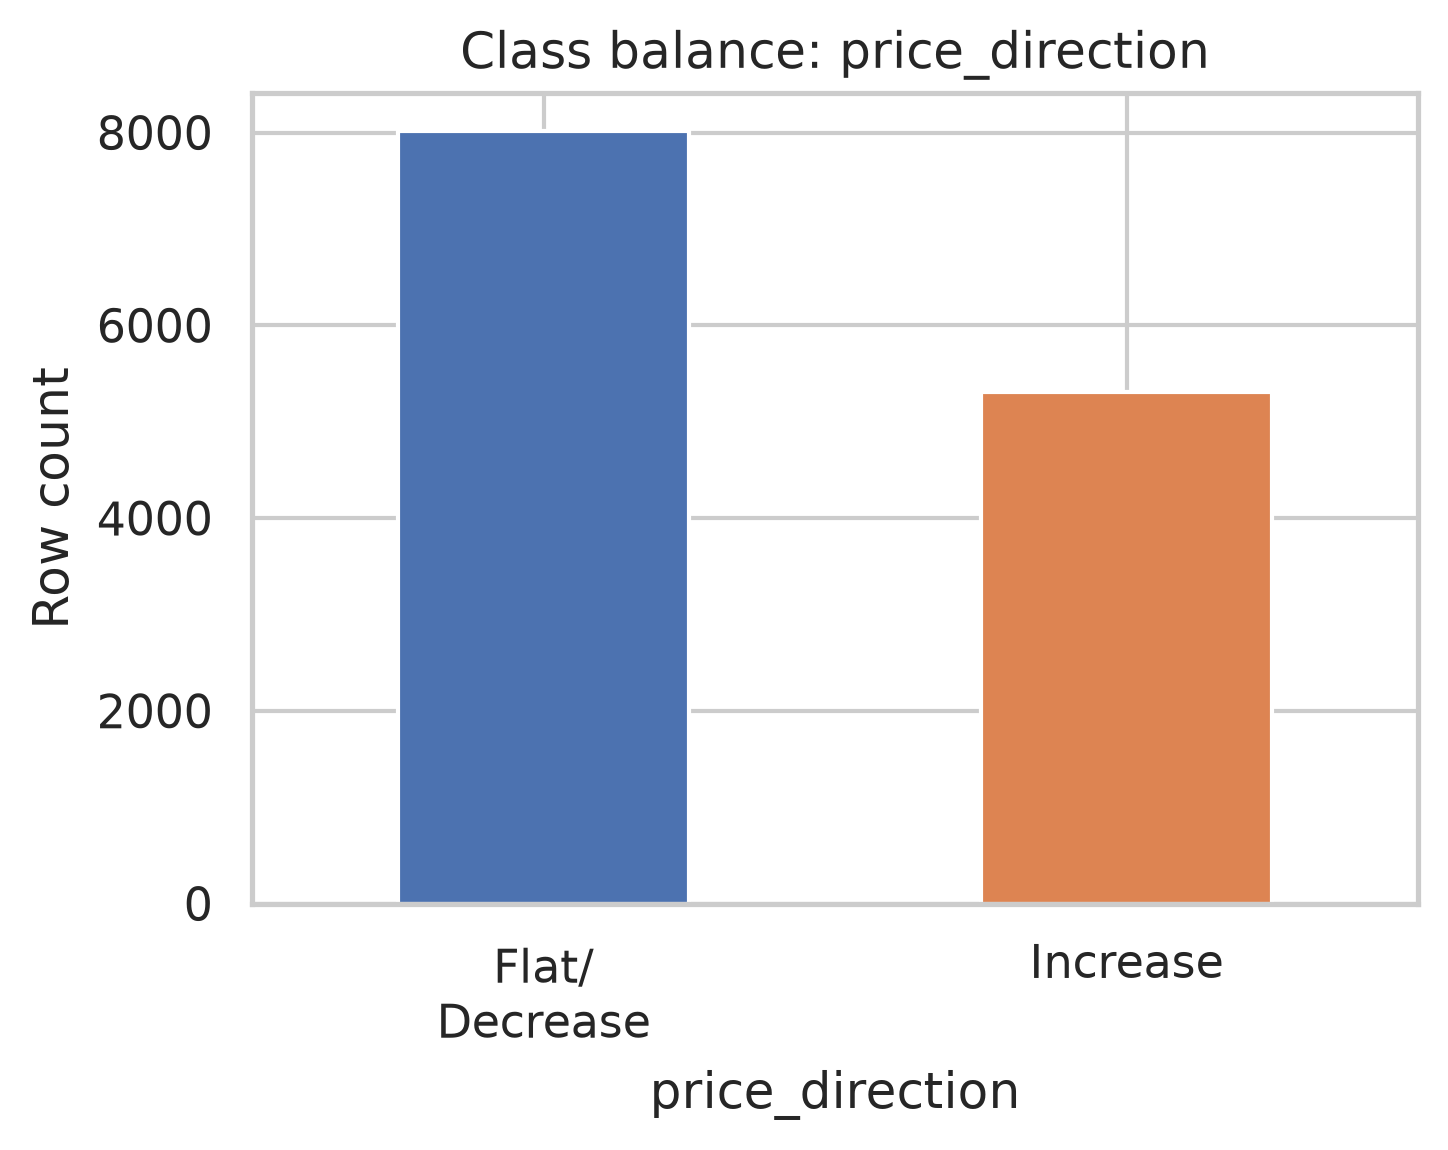
\includegraphics[width=0.5\textwidth]{price_direction_balance}
  \caption{Class balance of the classification target.}
  \label{fig:class_balance}
\end{figure}

\begin{figure}[H]
  \centering
  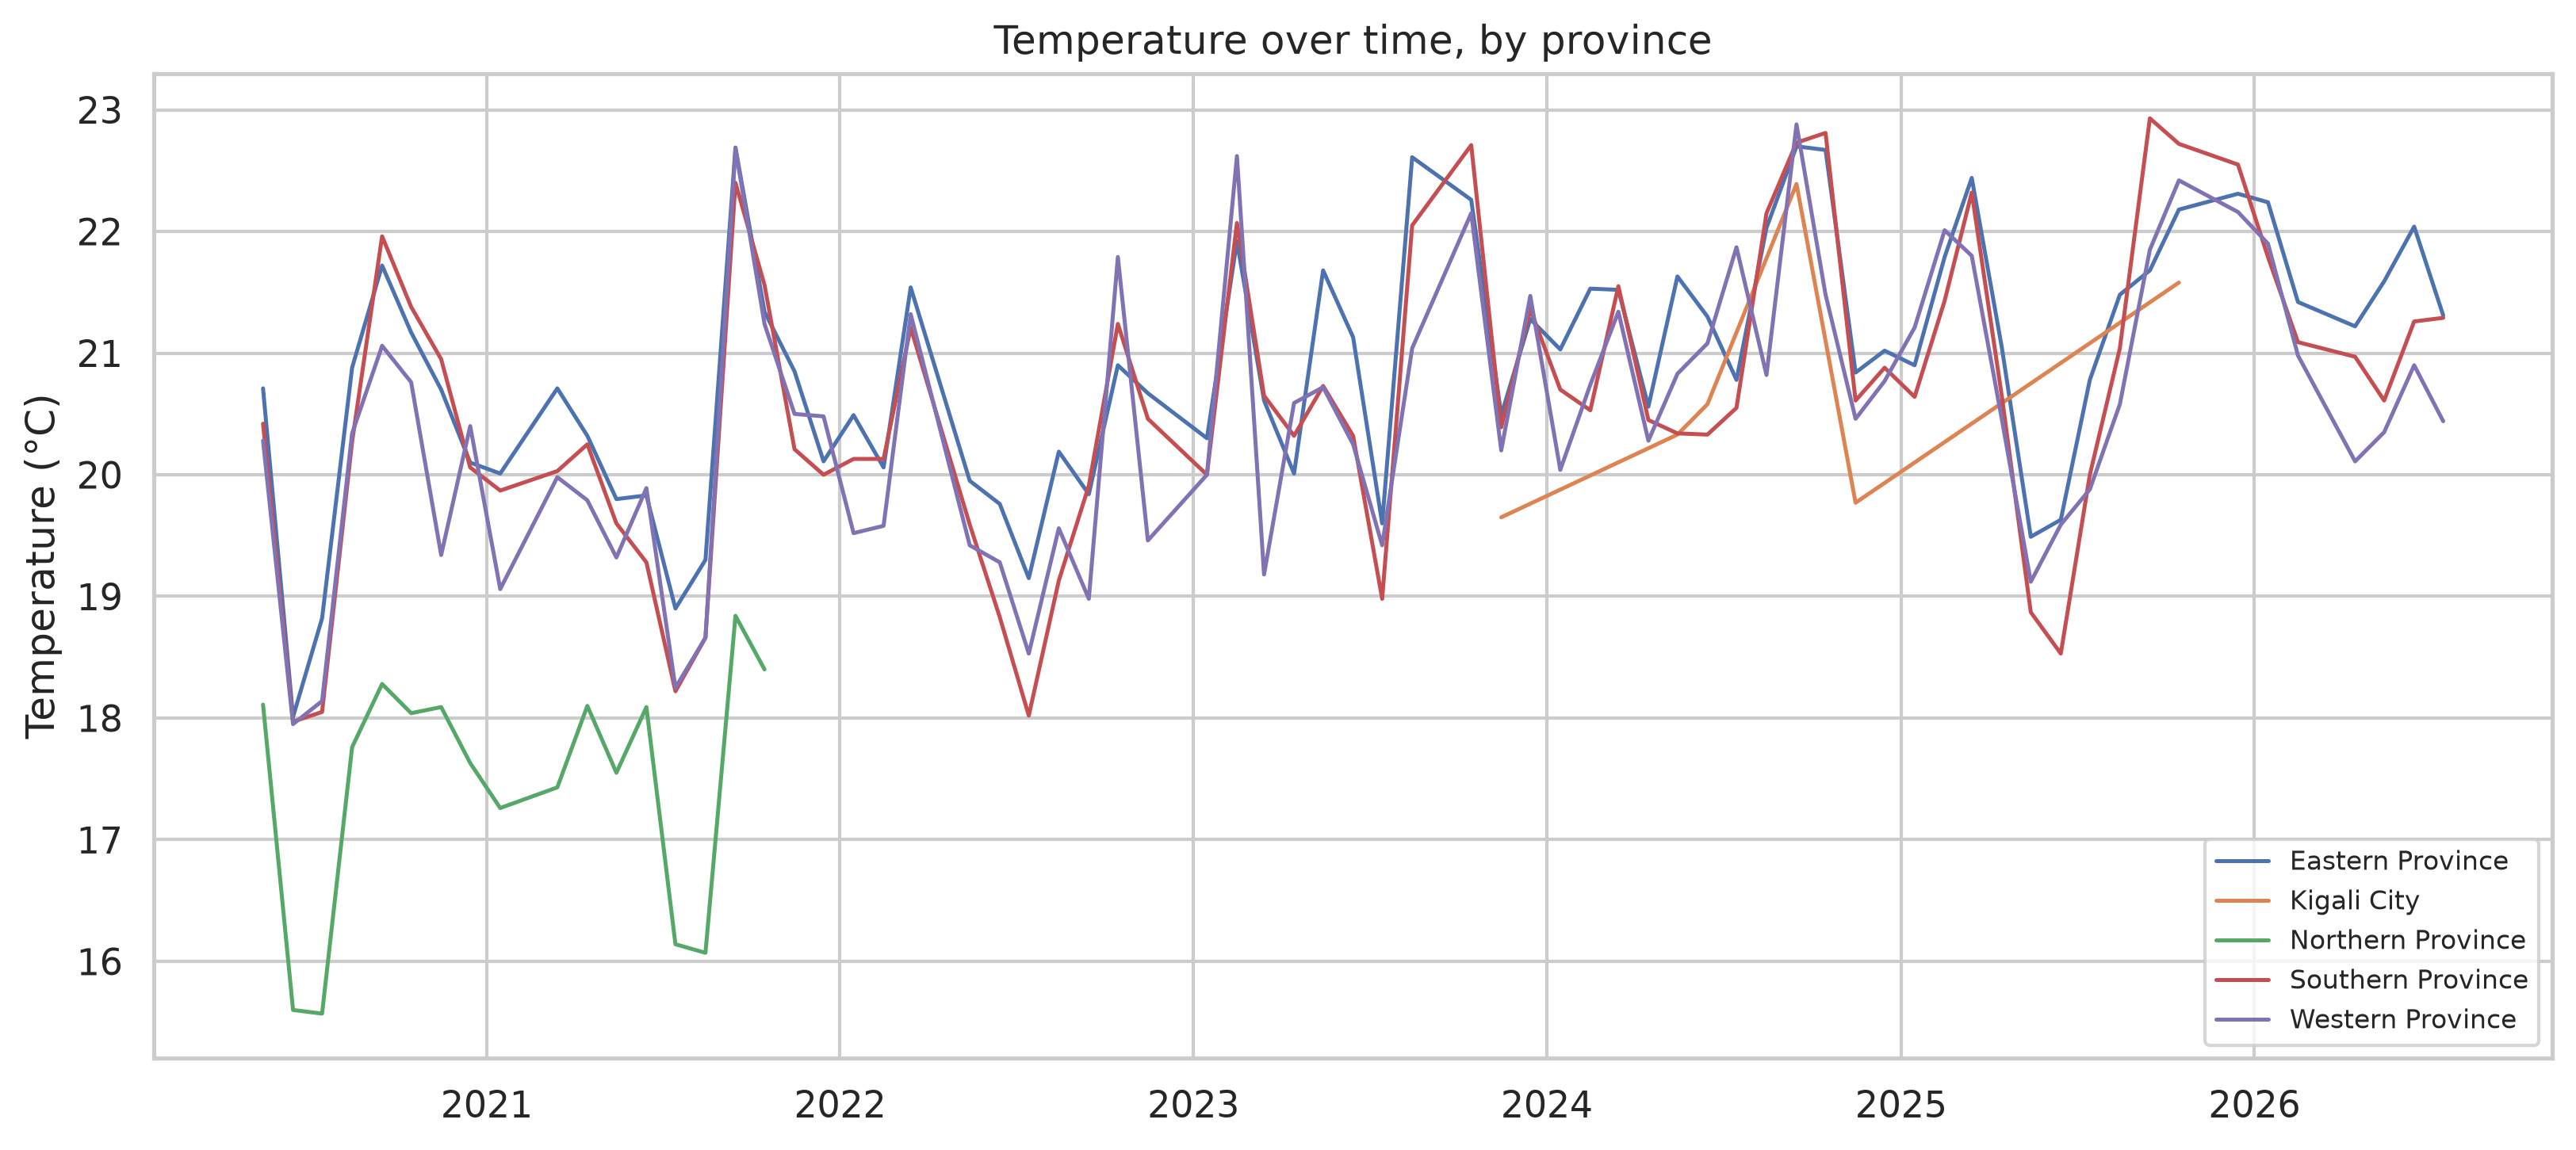
\includegraphics[width=0.85\textwidth]{temperature_by_province}
  \caption{Temperature over time by province. Kigali City's smooth line
  reflects very few distinct survey dates and should not be read as a
  seasonal trend.}
  \label{fig:temp_province}
\end{figure}

\begin{figure}[H]
  \centering
  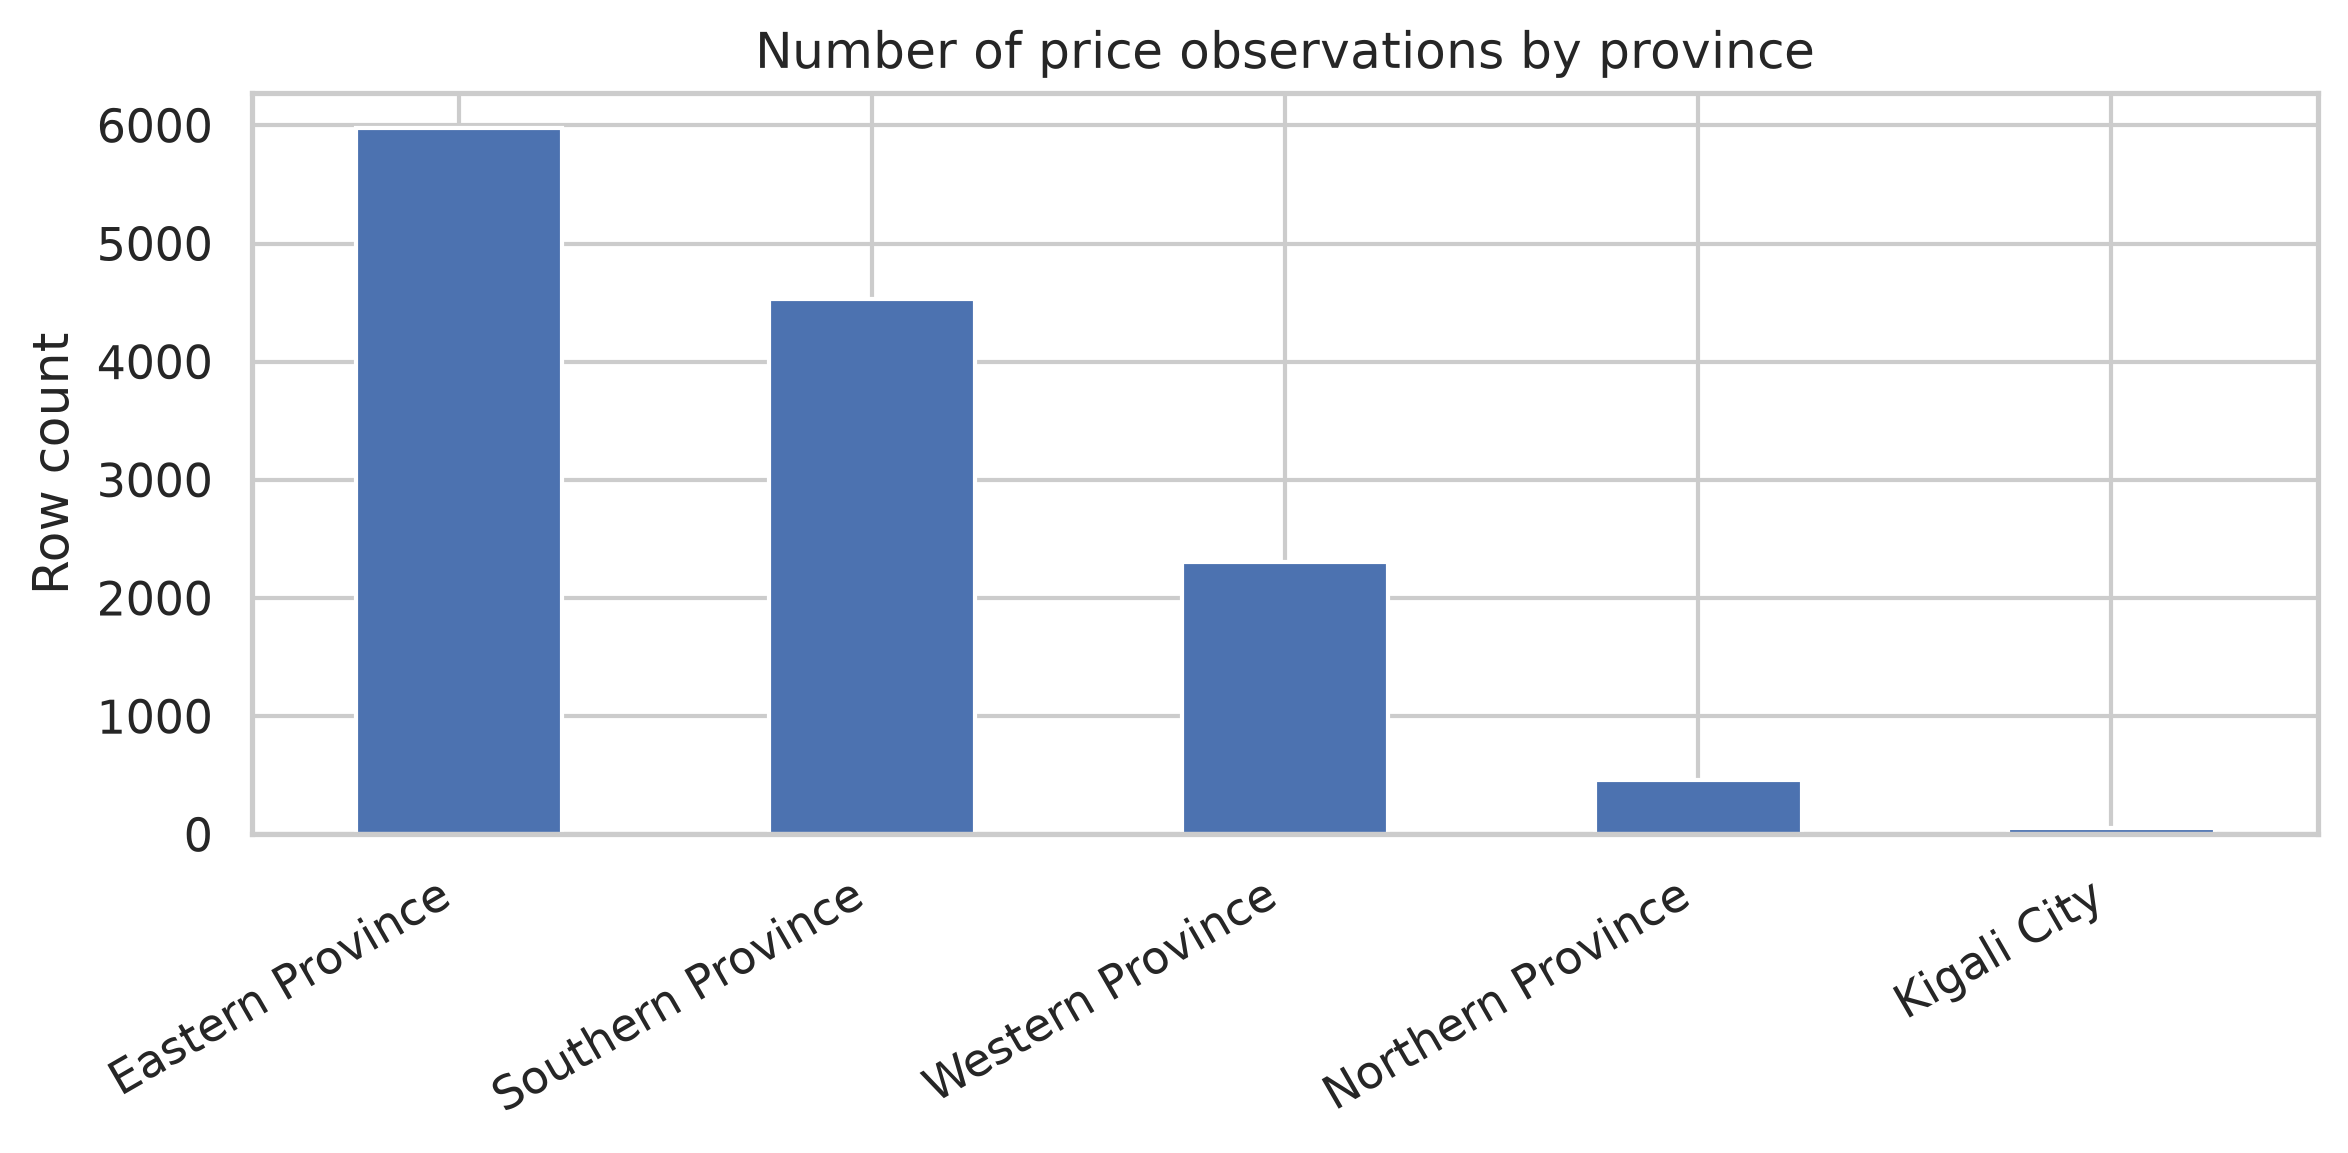
\includegraphics[width=0.7\textwidth]{observations_by_province}
  \caption{Price observations by province, illustrating uneven coverage.}
  \label{fig:obs_province}
\end{figure}

\begin{figure}[H]
  \centering
  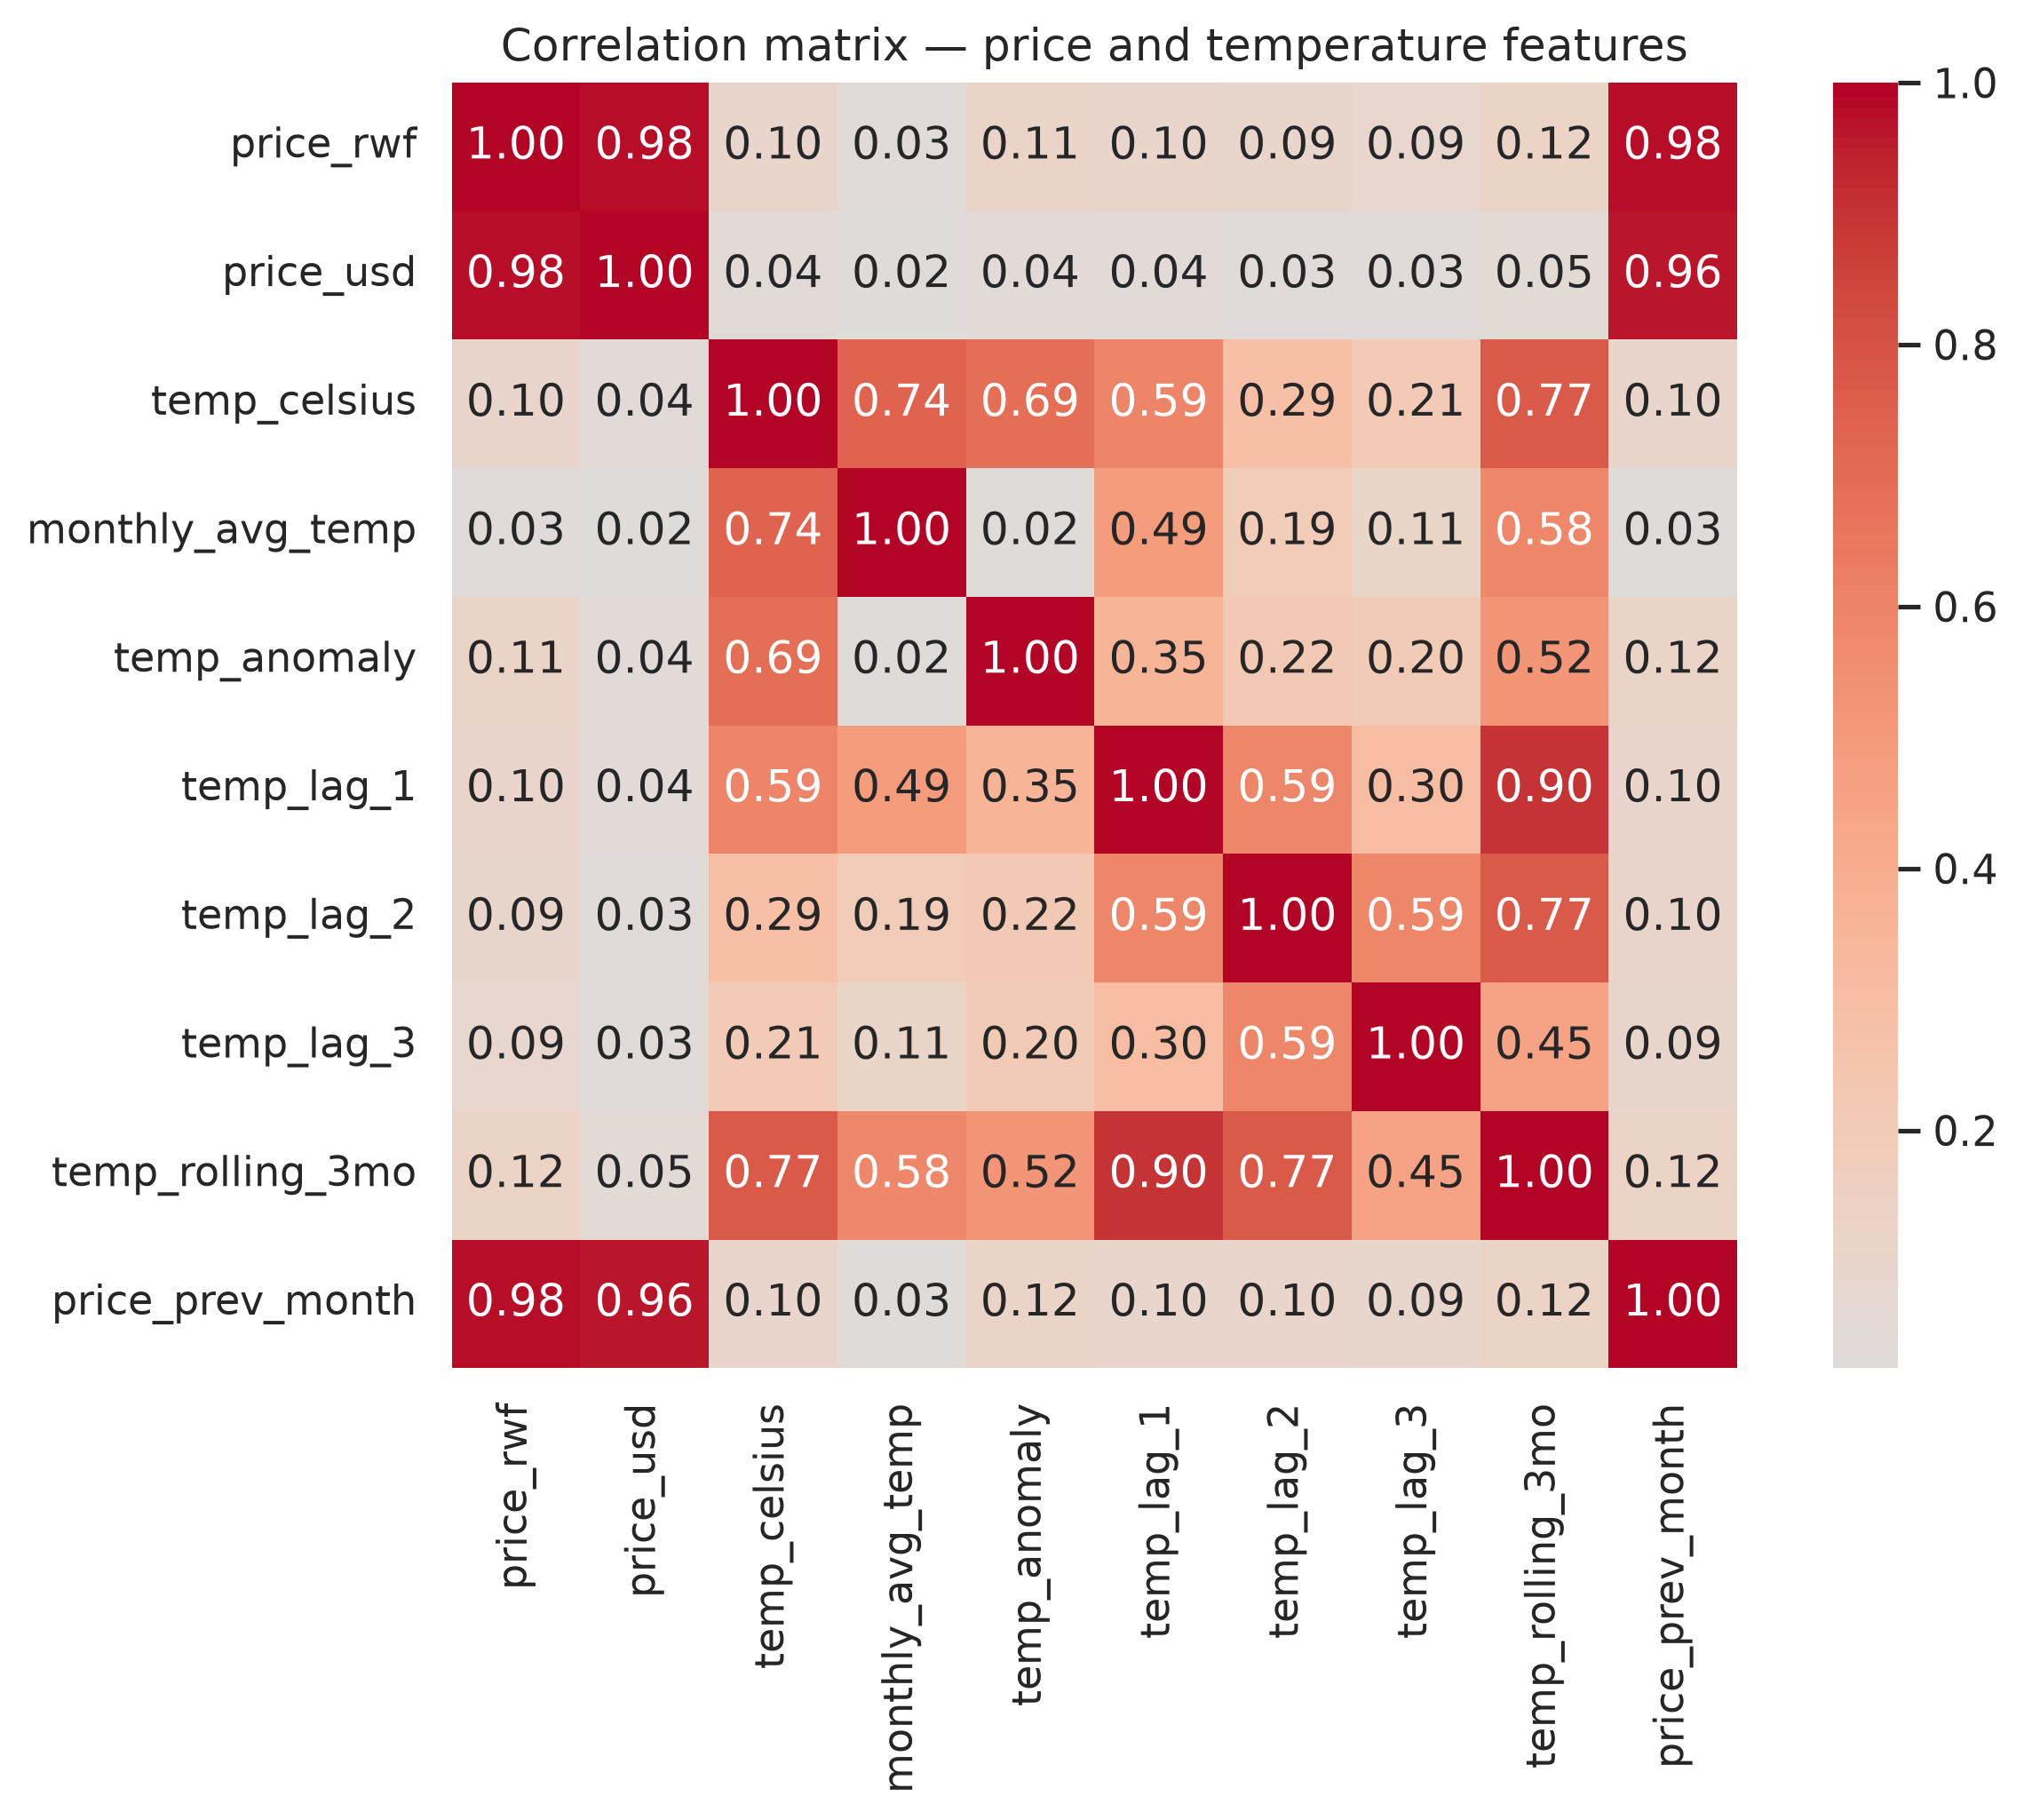
\includegraphics[width=0.75\textwidth]{correlation_heatmap}
  \caption{Correlation matrix of price and climate features.}
  \label{fig:corr_heatmap}
\end{figure}

\begin{figure}[H]
  \centering
  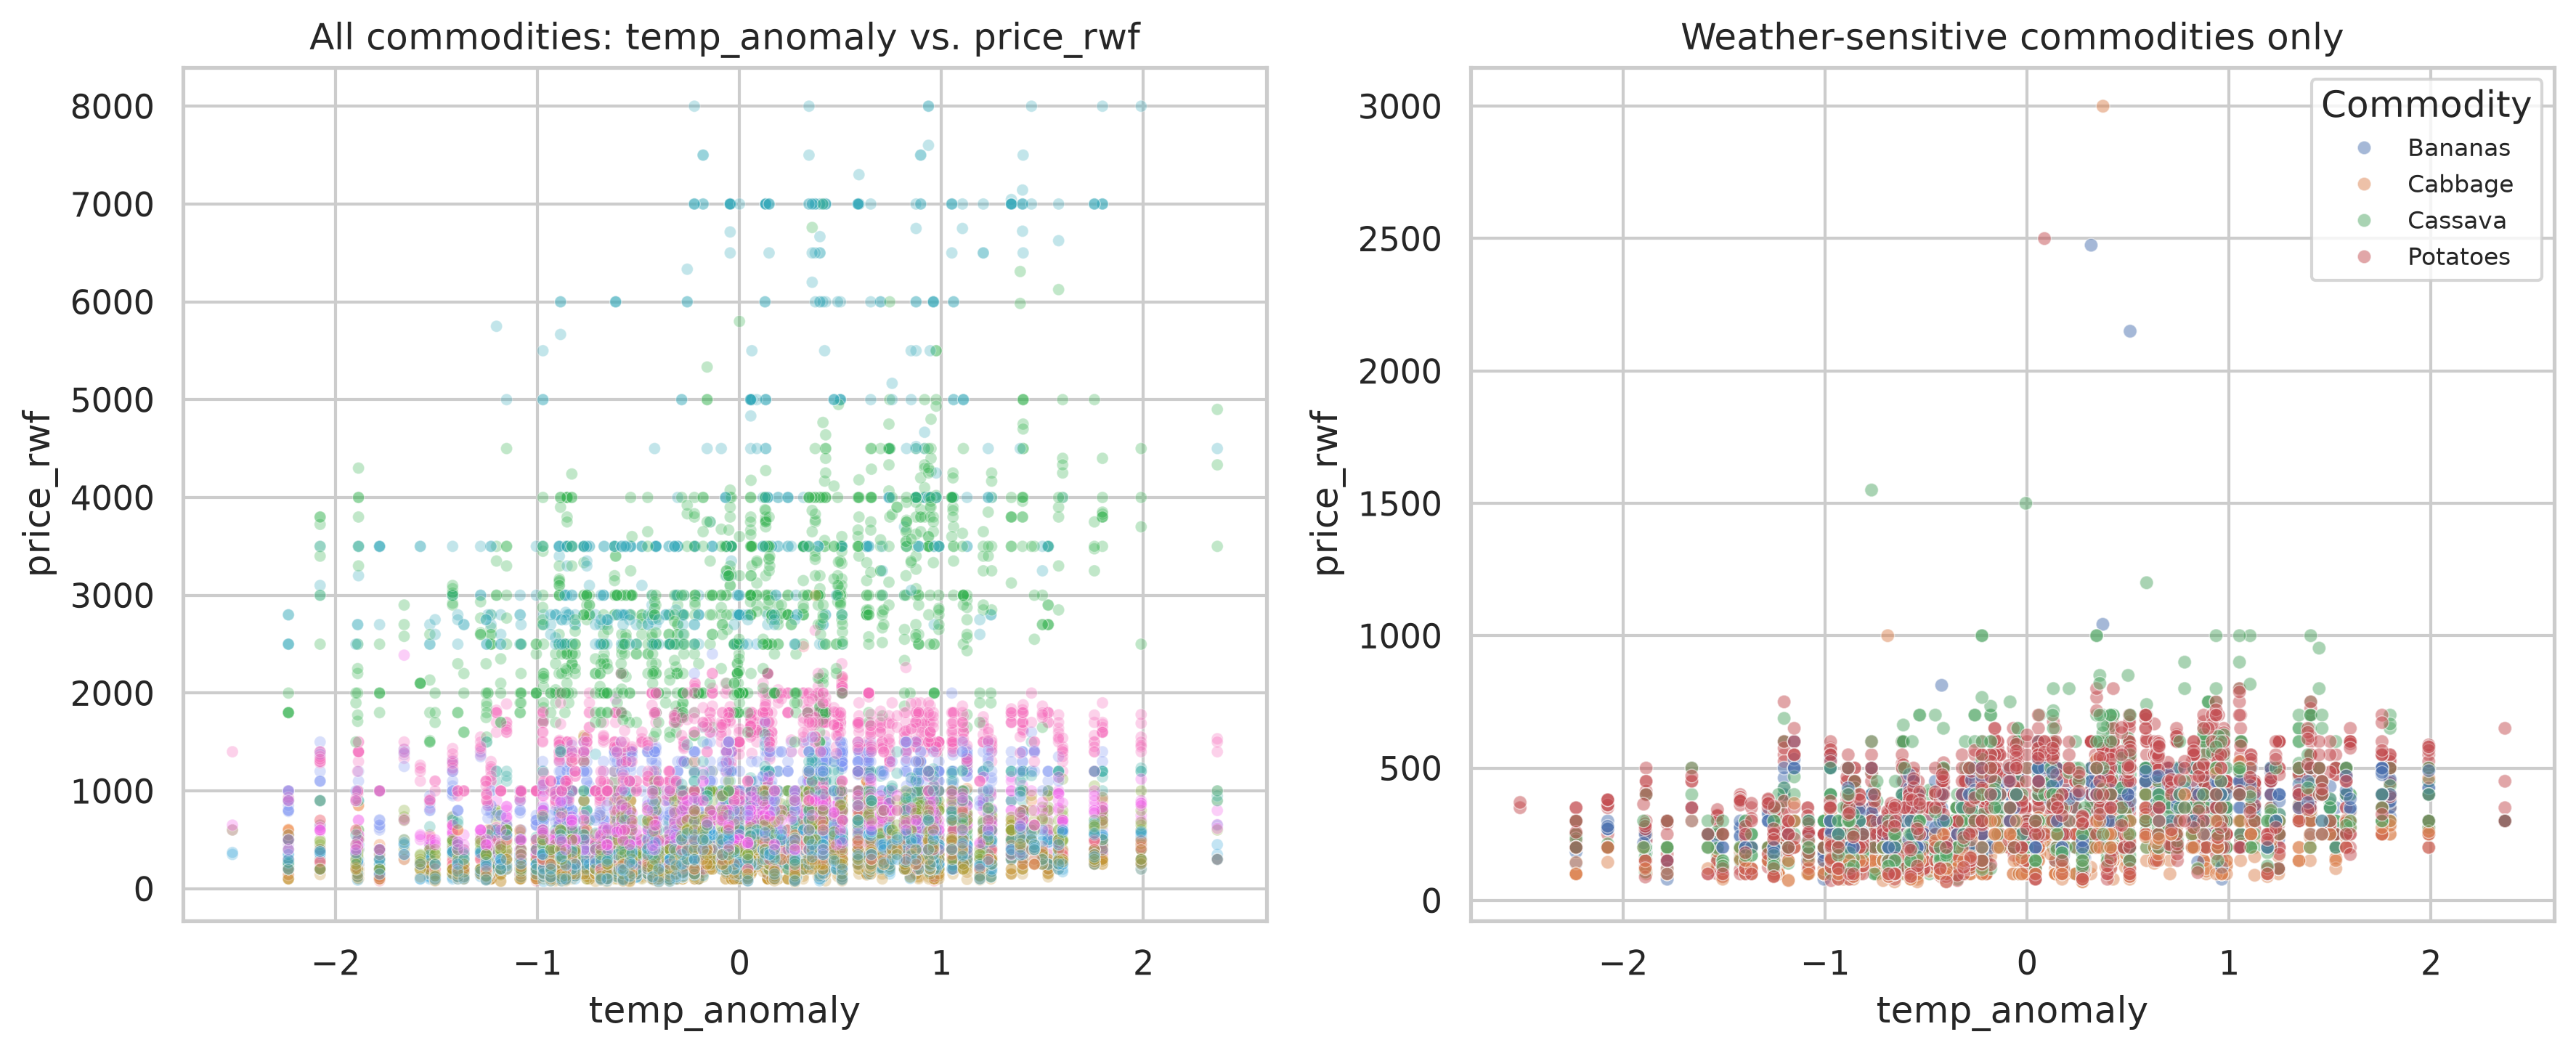
\includegraphics[width=0.85\textwidth]{temp_price_scatter_weathersensitive}
  \caption{Price versus temperature anomaly, all commodities (left) and
  weather-sensitive commodities only (right).}
  \label{fig:temp_scatter}
\end{figure}

\subsection{Feature Set}

The final feature set comprises \NFeatures{} input columns: four categorical (\texttt{province}, \texttt{market\_name}, \texttt{food\_category},
\texttt{commodity\_group}, one-hot encoded) and twelve numeric (standardised). The numeric features are the autoregressive baseline
(\texttt{price\_prev\_month}), a seasonality indicator (\texttt{month}), four macroeconomic series, and six climate variables.

The feature set was deliberately pruned from a larger candidate pool. Highly collinear pairs were reduced to one member each  general CPI was dropped in
favour of food CPI, and the redundant one- to three-month lag ladder was reduced to anomalies and rolling averages. \texttt{year} was excluded
specifically because of the chronological split: test-set years do not appear in training, and tree-based models cannot extrapolate beyond the range of a
feature they have seen, so including it would introduce a systematic disadvantage rather than useful signal.

Columns constant after cleaning (\texttt{country}, \texttt{unit}, \texttt{price\_flag}, \texttt{price\_type}, \texttt{currency}), redundant with
a retained coarser feature (\texttt{commodity\_name}, \texttt{district}), or directly leaking the target (\texttt{price\_usd}, a near-exact currency
conversion of \texttt{price\_rwf}) were excluded.

Note that the macroeconomic features vary only by date, so all rows sharing a survey date receive identical values. This is correct for an economy-wide
covariate and is not a leakage concern: the model learns how changes in a shared national series relate to an individual row's price behaviour.

\subsection{Train/Test Split and Cross-Validation}

Because the dataset is panel-structured  the same market--commodity pairs recur monthly  a random split would allow a model to observe a series'
future values during training and be evaluated on that same series' past. We use a \textbf{chronological split} at \CutoffDate{}: \NTrain{} training rows
from earlier dates and \NTest{} test rows from later ones. The same principle governs cross-validation during tuning, which uses \texttt{TimeSeriesSplit}
rather than random $k$-fold.

\subsection{Algorithms}

For both supervised tasks, four algorithms were compared: logistic/linear regression, random forest \citep{breiman2001random}, gradient boosting
\citep{friedman2001greedy}, and a multi-layer perceptron with three hidden layers (64, 32, 16 units) as the deep learning model, all implemented in
\texttt{scikit-learn} \citep{pedregosa2011scikit}. Each was compared against a naive baseline (majority-class classifier; mean-value regressor) to establish
whether a model learns anything beyond a trivial rule  a comparison that matters here, as Section~\ref{sec:results} shows.

All preprocessing is wrapped inside \texttt{Pipeline} objects so that encoders and scalers are fitted on training folds only, preventing leakage from
re-entering at the modelling stage after being removed during cleaning.

For clustering, market--commodity pairs with at least five observations (\NPairs{} pairs) were profiled by mean log-price, log-price volatility, mean
temperature, mean precipitation, mean soil moisture, and the proportion of month-over-month increases, then standardised. K-Means
\citep{macqueen1967kmeans}, Agglomerative clustering with Ward linkage \citep{ward1963hierarchical}, and a Gaussian mixture model
\citep{reynolds2009gmm} were compared, with $k$ selected by silhouette score \citep{rousseeuw1987silhouettes} and inter-algorithm agreement measured by the
Adjusted Rand Index \citep{hubert1985ari}. Exchange rate and CPI are excluded from the clustering features: they vary only by date, so they cannot
distinguish one market or commodity from another and would contribute noise reflecting \emph{when} a pair was observed rather than how it behaves.

\subsection{Problem Formulation and Model Specifications}
\label{sec:formulas}

Let $\mathbf{x}_i \in \mathbb{R}^{p}$ denote the feature vector for observation $i$ after one-hot encoding and standardisation, where standardisation applies
$z = (x - \hat{\mu})/\hat{\sigma}$ with $\hat{\mu}, \hat{\sigma}$ estimated on training folds only.

The two supervised targets are
\begin{align}
  y_i^{\text{clf}} &= \ind\!\left[\, p_{i,t} > p_{i,t-1} \,\right]
    \in \{0, 1\}, \\
  y_i^{\text{reg}} &= \log\!\left(1 + p_{i,t}\right),
\end{align}
where $p_{i,t}$ is the price in RWF/kg of a given commodity at a given market in month $t$. Regression predictions are reported on the original scale via
the inverse transform $\hat{p} = \exp(\hat{y}) - 1$, which is why RMSE and MAE appear in RWF while $R^2$ is quoted on the log scale.

\paragraph{Logistic regression.} Models the conditional probability through the logistic link and is fitted by penalised maximum likelihood:
\begin{equation}
  \Pr(y = 1 \mid \mathbf{x}) = \sigma(\beta_0 + \boldsymbol{\beta}^\top \mathbf{x}),
  \qquad \sigma(z) = \frac{1}{1 + e^{-z}},
\end{equation}
\begin{equation}
  \hat{\boldsymbol{\beta}} = \arg\min_{\boldsymbol{\beta}}
  \; \frac{1}{2}\lVert \boldsymbol{\beta} \rVert_2^{2}
  + C \sum_{i=1}^{n} \log\!\left(1 + e^{-\tilde{y}_i (\beta_0 + \boldsymbol{\beta}^\top \mathbf{x}_i)}\right),
\end{equation}
with $\tilde{y}_i \in \{-1, +1\}$ and $C$ the inverse regularisation strength.

\paragraph{Linear regression.} Minimises the residual sum of squares on the log-transformed target:
\begin{equation}
  \hat{\boldsymbol{\beta}} = \arg\min_{\boldsymbol{\beta}}
  \sum_{i=1}^{n}\left(y_i - \beta_0 - \boldsymbol{\beta}^\top \mathbf{x}_i\right)^{2}.
\end{equation}

\paragraph{Random forest.} Averages $B$ trees grown on bootstrap resamples, each split selecting from a random subset of $m$ features
\citep{breiman2001random}:
\begin{equation}
  \hat{f}_{\text{reg}}(\mathbf{x}) = \frac{1}{B}\sum_{b=1}^{B} T_b(\mathbf{x}),
  \qquad
  \hat{f}_{\text{clf}}(\mathbf{x}) = \arg\max_{k}\;\frac{1}{B}\sum_{b=1}^{B}\hat{p}_{b,k}(\mathbf{x}).
\end{equation}
Splits maximise impurity reduction, using Gini impurity for classification and squared-error reduction for regression:
\begin{equation}
  G = \sum_{k} \hat{p}_k\left(1 - \hat{p}_k\right),
  \qquad
  \text{SSE} = \sum_{i \in R}\left(y_i - \bar{y}_R\right)^{2}.
\end{equation}
Randomising $m$ decorrelates the trees, so averaging reduces variance more than bagging alone. The tuned regressor selected $m = \lceil 0.5p \rceil$
(\texttt{max\_features}~$=0.5$).

\paragraph{Gradient boosting.} Fits an additive model stagewise, each stage correcting its predecessor along the negative gradient of the loss
\citep{friedman2001greedy}:
\begin{equation}
  F_0(\mathbf{x}) = \arg\min_{\gamma}\sum_{i=1}^{n} L(y_i, \gamma),
  \qquad
  F_m(\mathbf{x}) = F_{m-1}(\mathbf{x}) + \nu\, h_m(\mathbf{x}),
\end{equation}
where $h_m$ is a regression tree fitted to the pseudo-residuals
\begin{equation}
  r_{im} = -\left[\frac{\partial L\!\left(y_i, F(\mathbf{x}_i)\right)}{\partial F(\mathbf{x}_i)}\right]_{F = F_{m-1}},
\end{equation}
$\nu$ is the learning rate, $L$ is squared error for regression and log-loss for classification. Boosting reduces bias sequentially, whereas the random
forest reduces variance in parallel  which is why the two behave differently here despite both being tree ensembles.

\paragraph{Multi-layer perceptron.} A feed-forward network with three hidden layers of $(64, 32, 16)$ units and ReLU activations:
\begin{equation}
  \mathbf{h}^{(1)} = g\!\left(W^{(1)}\mathbf{x} + \mathbf{b}^{(1)}\right),
  \quad
  \mathbf{h}^{(l)} = g\!\left(W^{(l)}\mathbf{h}^{(l-1)} + \mathbf{b}^{(l)}\right),
  \quad
  g(z) = \max(0, z).
\end{equation}
The output layer applies $\sigma(\cdot)$ for classification and the identity for regression. Parameters minimise the task loss with an $L_2$ penalty of
weight $\alpha$,
\begin{equation}
  \min_{\{W, \mathbf{b}\}} \; \frac{1}{n}\sum_{i=1}^{n} L\!\left(y_i, \hat{y}_i\right)
  + \frac{\alpha}{2}\sum_{l}\lVert W^{(l)}\rVert_F^{2},
\end{equation}
optimised by Adam with early stopping on a held-out fraction of the training data.

\paragraph{K-Means.} Minimises within-cluster sum of squares:
\begin{equation}
  \min_{C_1,\dots,C_K}\;\sum_{k=1}^{K}\sum_{i \in C_k}
  \lVert \mathbf{x}_i - \boldsymbol{\mu}_k \rVert_2^{2},
  \qquad
  \boldsymbol{\mu}_k = \frac{1}{|C_k|}\sum_{i \in C_k}\mathbf{x}_i .
\end{equation}
The squared Euclidean objective is what makes K-Means favour compact, isotropic clusters  relevant to the algorithm-agreement result in
Section~\ref{sec:results}.

\paragraph{Ward linkage.} Agglomerative merging of the pair whose union increases within-cluster variance least \citep{ward1963hierarchical}:
\begin{equation}
  d(A, B) = \frac{|A|\,|B|}{|A| + |B|}\,
  \lVert \boldsymbol{\mu}_A - \boldsymbol{\mu}_B \rVert_2^{2}.
\end{equation}
Ward optimises essentially the same variance criterion as K-Means, which explains their near-identical partitions here.

\paragraph{Gaussian mixture model.} Models the data as a mixture of $K$ Gaussian components with individual covariances \citep{reynolds2009gmm}:
\begin{equation}
  p(\mathbf{x}) = \sum_{k=1}^{K}\pi_k\,
  \mathcal{N}\!\left(\mathbf{x} \mid \boldsymbol{\mu}_k, \Sigma_k\right),
  \qquad \sum_{k}\pi_k = 1,
\end{equation}
fitted by expectation-maximisation. Because $\Sigma_k$ is unconstrained, the GMM admits elliptical clusters of differing orientation and volume; this is the
formal reason it can disagree with K-Means and Ward on data whose true structure is spherical.

\subsection{Evaluation Metrics}
\label{sec:metrics}

With $TP$, $FP$, $TN$, $FN$ the confusion-matrix counts for the positive class (``price increased''):
\begin{equation}
  \text{Precision} = \frac{TP}{TP + FP},
  \qquad
  \text{Recall} = \frac{TP}{TP + FN},
  \qquad
  F_1 = \frac{2\,\text{Precision}\cdot\text{Recall}}{\text{Precision} + \text{Recall}} .
\end{equation}
ROC-AUC is the area under the curve traced by the true-positive against false-positive rate as the decision threshold varies, equivalently the
probability that a randomly chosen positive is ranked above a randomly chosen negative. It is therefore threshold-independent, whereas $F_1$ is evaluated at
a single threshold (0.5 by default)  a distinction that matters directly for the ablation in Section~\ref{sec:ablation}.

For regression, with predictions back-transformed to RWF:
\begin{equation}
  \text{RMSE} = \sqrt{\frac{1}{n}\sum_{i=1}^{n}\left(y_i - \hat{y}_i\right)^{2}},
  \quad
  \text{MAE} = \frac{1}{n}\sum_{i=1}^{n}\left|y_i - \hat{y}_i\right|,
  \quad
  R^{2} = 1 - \frac{\sum_i (y_i - \hat{y}_i)^{2}}{\sum_i (y_i - \bar{y})^{2}} .
\end{equation}

For clustering, the silhouette coefficient for point $i$ is
\begin{equation}
  s(i) = \frac{b(i) - a(i)}{\max\{a(i),\, b(i)\}} \in [-1, 1],
\end{equation}
with $a(i)$ the mean distance to points in its own cluster and $b(i)$ the mean distance to the nearest other cluster. The Adjusted Rand Index compares two
partitions, correcting for chance agreement \citep{hubert1985ari}:
\begin{equation}
  \text{ARI} = \frac{\text{RI} - \mathbb{E}[\text{RI}]}{\max(\text{RI}) - \mathbb{E}[\text{RI}]},
\end{equation}
taking the value 1 for identical partitions and 0 for agreement no better than chance.

\subsection{Model Improvement}

The strongest baseline per task was tuned with \texttt{RandomizedSearchCV} under \texttt{TimeSeriesSplit} cross-validation. An earlier iteration produced
the counter-intuitive result that tuning \emph{degraded} test-set regression performance. The cause was a defect in the search space rather than in the
data: the random forest baseline used \texttt{max\_depth=12, min\_samples\_leaf=1}, while the grid offered only
\texttt{max\_depth} $\in \{6,10,15\}$ and \texttt{min\_samples\_leaf} $\in \{2,4\}$. The baseline configuration was unreachable, so the search could not
recover it, and a search that cannot return its own starting point will eventually appear to regress. The corrected grids contain each baseline
configuration, and the tuning routine additionally reports baseline and tuned scores under the \emph{same} cross-validation protocol, so that the comparison
is like-for-like and the test set is used only once, for final reporting.

\section{Results and Interpretation}
\label{sec:results}

\subsection{Classification: Predicting Price Direction}

Table~\ref{tab:classification} reports test-set performance. Every model beats the majority-class baseline on F1, but discrimination remains modest: the best
baseline ROC-AUC is 0.610, against 0.5 for a non-discriminative classifier. The random forest achieves the best baseline F1 (0.479) and is carried forward
for tuning as \BestClf{}.

Accuracy is actively misleading here. The majority-class baseline attains 0.584 accuracy while scoring precision, recall, and F1 of exactly zero on the
minority class  it achieves that accuracy purely by never predicting an increase. Logistic regression's accuracy (0.588) barely exceeds it despite
being substantially more useful. This is precisely why the evaluation protocol was fixed in advance on the basis of the observed class imbalance, rather than
chosen after seeing which metric was most flattering.

% AUTO-GENERATED by 3a_supervised_learning.ipynb -- do not edit by hand.
\begin{table}[H]
\centering
\caption{Classification performance on the chronological test set (2,606 rows).}
\label{tab:classification}
\begin{tabular}{lccccc}
\toprule
 & Accuracy & Precision & Recall & F1 & ROC-AUC \\
Model &  &  &  &  &  \\
\midrule
Dummy (majority class) & 0.584 & 0.000 & 0.000 & 0.000 & 0.500 \\
Logistic Regression & 0.588 & 0.507 & 0.422 & 0.461 & 0.588 \\
Random Forest & 0.607 & 0.535 & 0.434 & 0.479 & 0.608 \\
Gradient Boosting & 0.604 & 0.531 & 0.418 & 0.467 & 0.610 \\
MLP (deep learning) & 0.604 & 0.536 & 0.360 & 0.431 & 0.610 \\
\bottomrule
\end{tabular}
\end{table}


\begin{figure}[H]
  \centering
  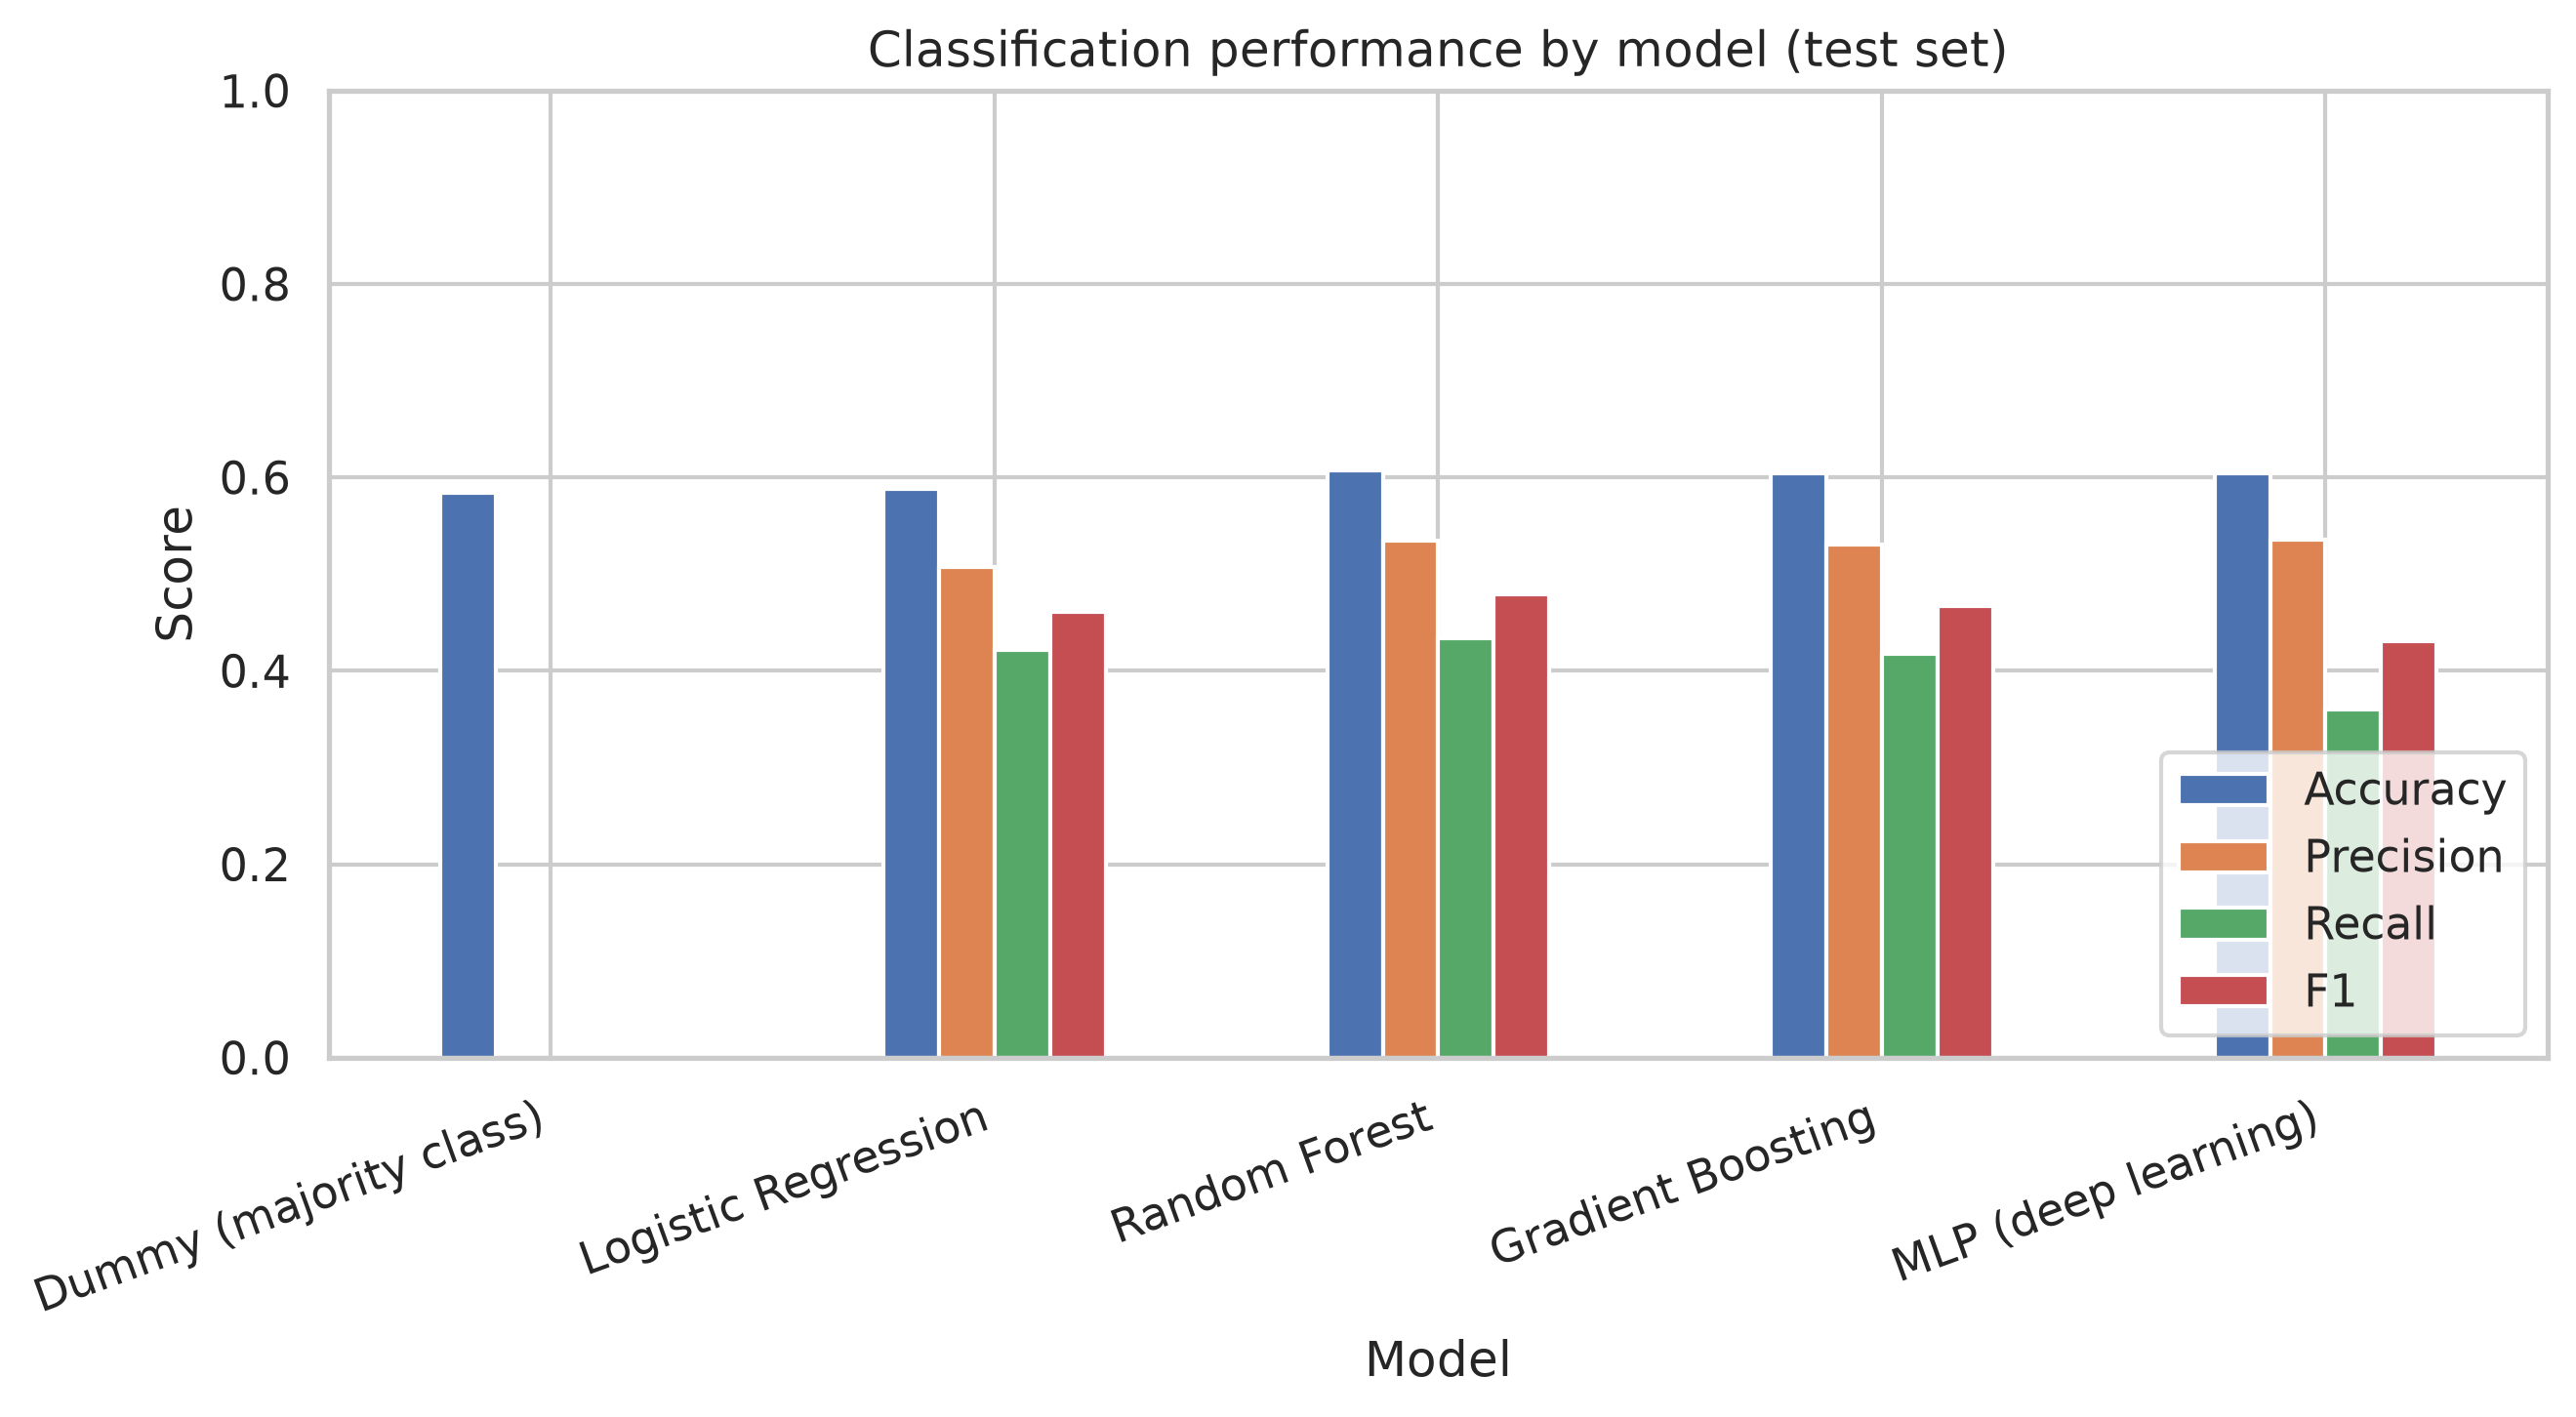
\includegraphics[width=0.85\textwidth]{classification_model_comparison}
  \caption{Classification performance by model on the test set.}
  \label{fig:clf_compare}
\end{figure}

\begin{figure}[H]
  \centering
  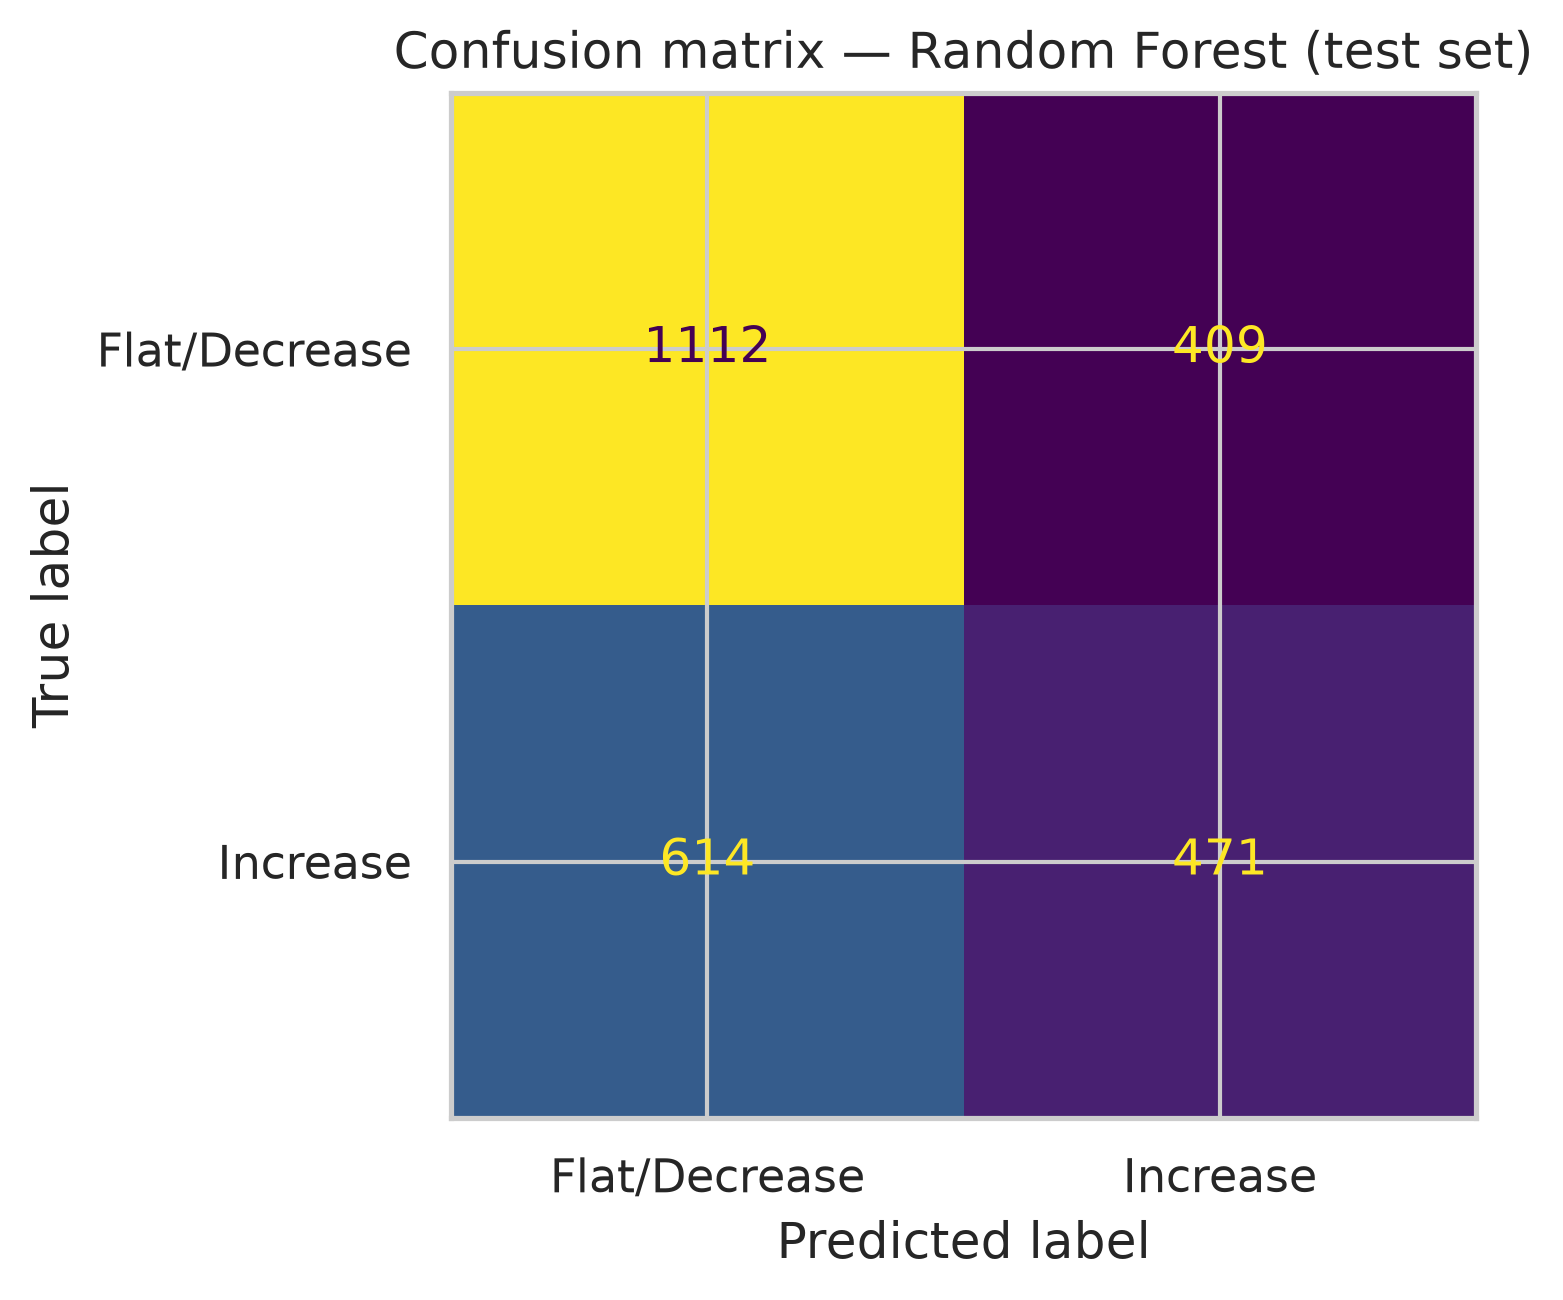
\includegraphics[width=0.5\textwidth]{confusion_matrix_best_classifier}
  \caption{Confusion matrix for the best baseline classifier.}
  \label{fig:confusion}
\end{figure}

\subsection{Regression: Predicting Price Level}

Table~\ref{tab:regression} reports test-set performance. Measured against the mean-prediction baseline, the results appear strong: the random forest attains
$R^2 = 0.94$ on the log-transformed target and an RMSE of 466 RWF against 1{,}747 RWF, an apparent 73\% reduction in error.

That comparison, however, uses the wrong null model. \texttt{DummyRegressor} predicts the global mean price and therefore ignores the most obvious
forecasting rule available for a time series: that next month's price is usually close to this month's. The appropriate benchmark is a \textbf{naive
persistence forecast}  carry the previous month's price forward unchanged, using no training and no features.

\textbf{No trained model beats it.} Persistence achieves RMSE 295 RWF and MAE 124 RWF, against 466 and 193 for the best random forest; the ensemble's error
is roughly 58\% \emph{higher} than simply repeating last month's price (Figure~\ref{fig:persistence}). The near-identical $R^2$ values are themselves
misleading: on the log scale $R^2$ is dominated by variance \emph{between} commodities  beef trades near 3{,}500 RWF/kg and cabbage near 200  which
persistence and the trained models both capture trivially. Decomposing the sources of fit makes this explicit: predicting the global mean yields
$R^2 = -0.15$, commodity identity alone yields $0.71$, and last month's price alone yields $0.944$, which is precisely what the tuned random forest achieves.

The honest conclusion is that the apparently high regression performance reflects price autocorrelation and commodity-level price separation rather
than forecasting skill. This does not invalidate the exercise  the pipeline, the leakage controls, and the algorithm comparison all stand  but it bounds
what may be claimed from it: for predicting price \emph{levels} in this dataset, a zero-parameter rule outperforms every algorithm compared here.

Feature importance (Figure~\ref{fig:importance}) is consistent with this reading: the model relies overwhelmingly on \texttt{price\_prev\_month} and
commodity identity, which is to say it has largely learned to approximate the persistence rule while adding variance of its own.

The multi-layer perceptron is the weakest non-trivial regressor (RMSE 636 RWF) and does not lead on classification either. Neural networks
hold no inherent advantage on small, structured tabular data of this kind, where ensemble methods that partition feature space directly are typically
stronger. Including a deep learning model satisfies the assignment brief and makes a useful comparison, but the honest reading is that it is not the right
tool for this dataset at this scale.

% AUTO-GENERATED by 3a_supervised_learning.ipynb -- do not edit by hand.
\begin{table}[H]
\centering
\caption{Regression performance on the chronological test set (original-scale RWF unless noted), including a naive persistence baseline.}
\label{tab:regression}
\begin{tabular}{lccc}
\toprule
 & RMSE (RWF) & MAE (RWF) & R2 (log scale) \\
Model &  &  &  \\
\midrule
Naive persistence (last month's price) & 295.30 & 124.18 & 0.94 \\
Dummy (mean) & 1746.83 & 863.60 & -0.15 \\
Linear Regression & 775.00 & 308.84 & 0.91 \\
Random Forest & 465.21 & 192.08 & 0.94 \\
Gradient Boosting & 496.44 & 197.22 & 0.94 \\
MLP (deep learning) & 635.87 & 361.44 & 0.85 \\
\bottomrule
\end{tabular}
\end{table}


\begin{figure}[H]
  \centering
  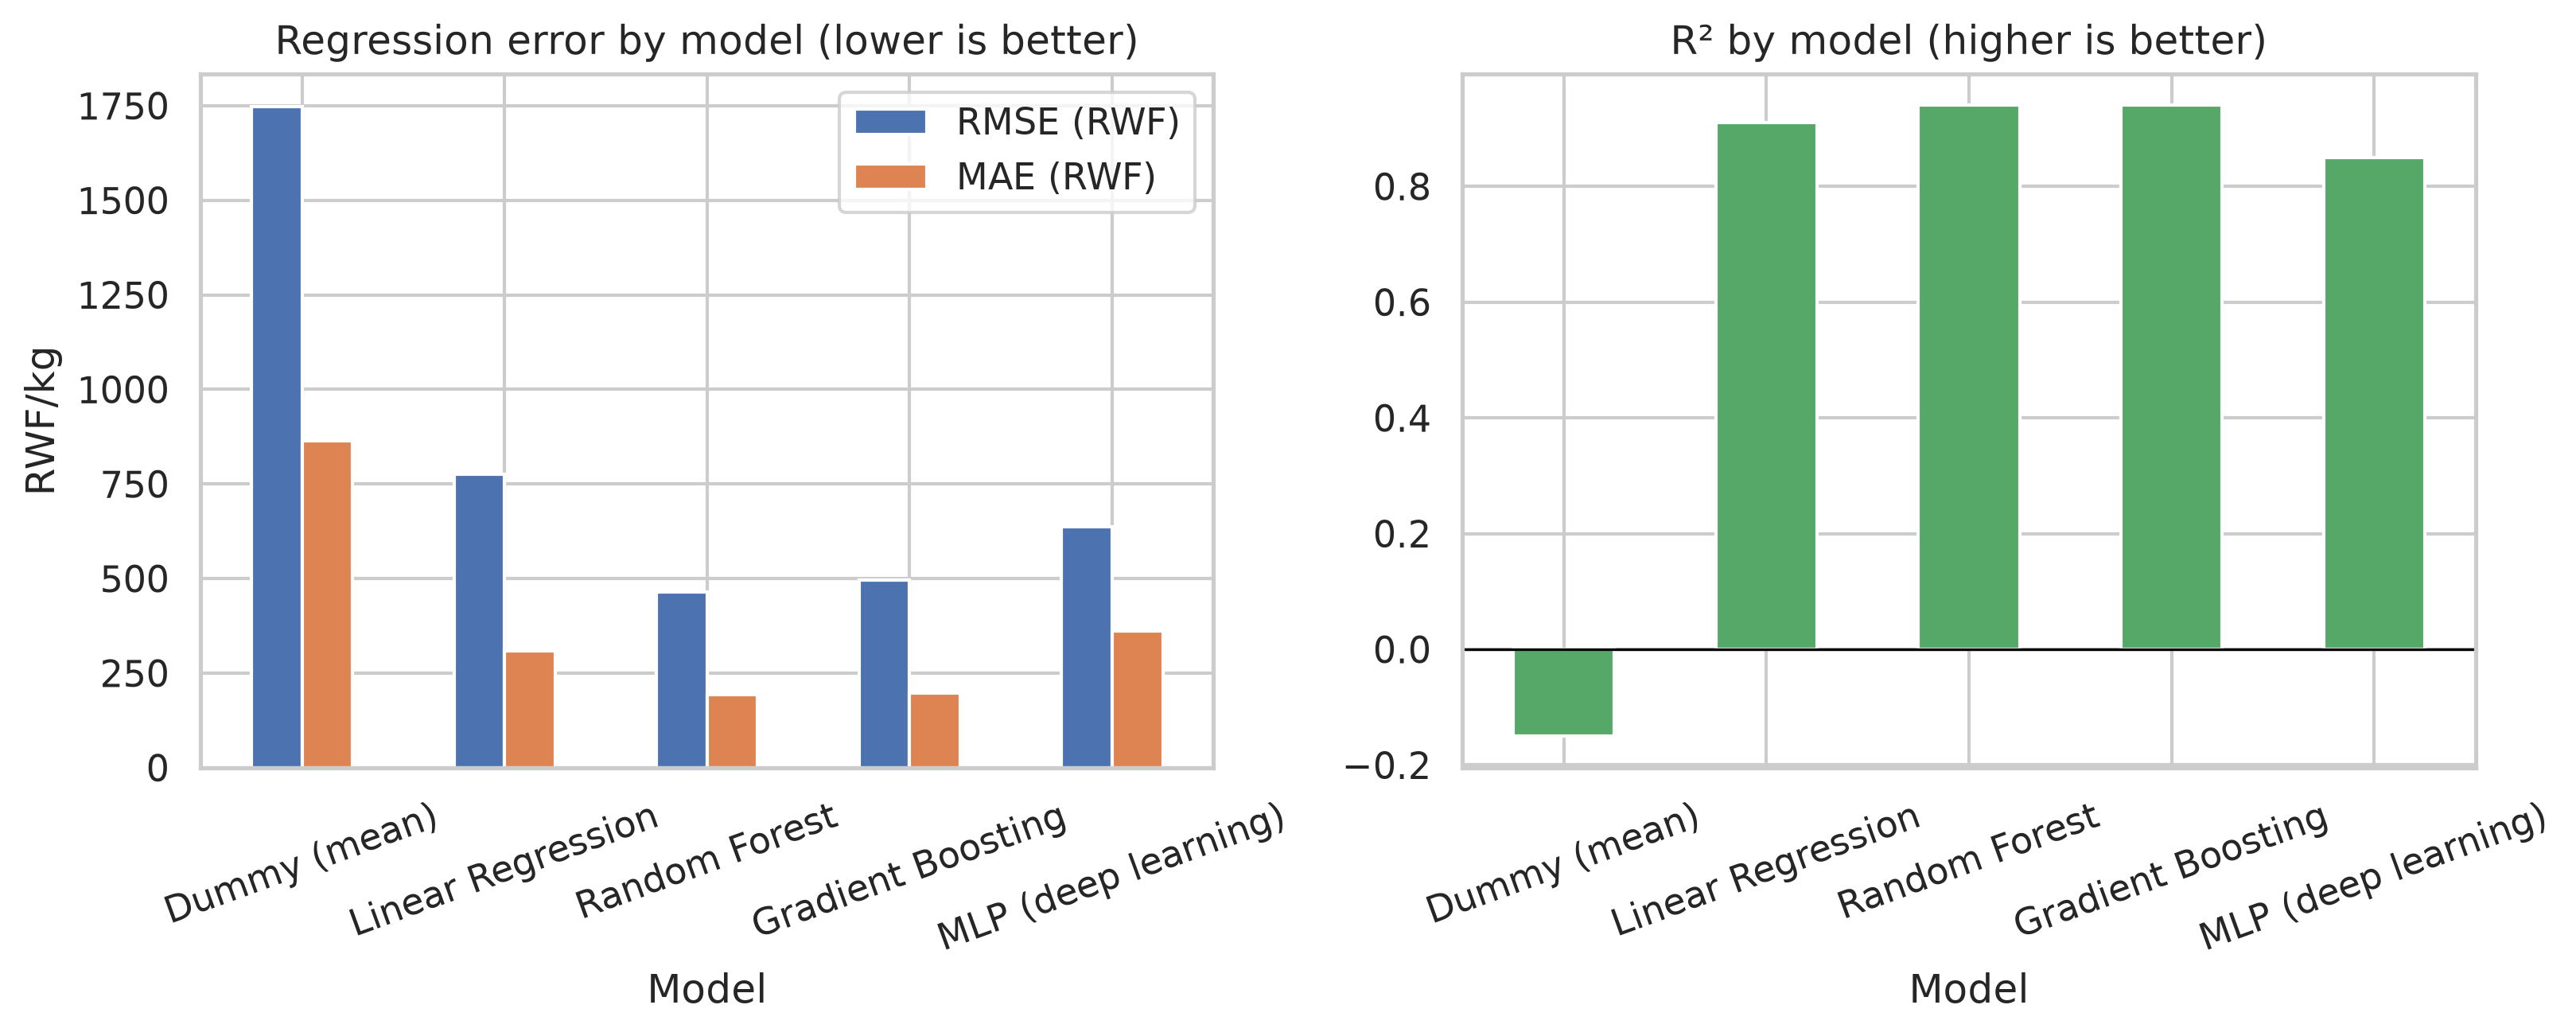
\includegraphics[width=0.85\textwidth]{regression_model_comparison}
  \caption{Regression error (RMSE, MAE) and $R^2$ by model.}
  \label{fig:reg_compare}
\end{figure}

\begin{figure}[H]
  \centering
  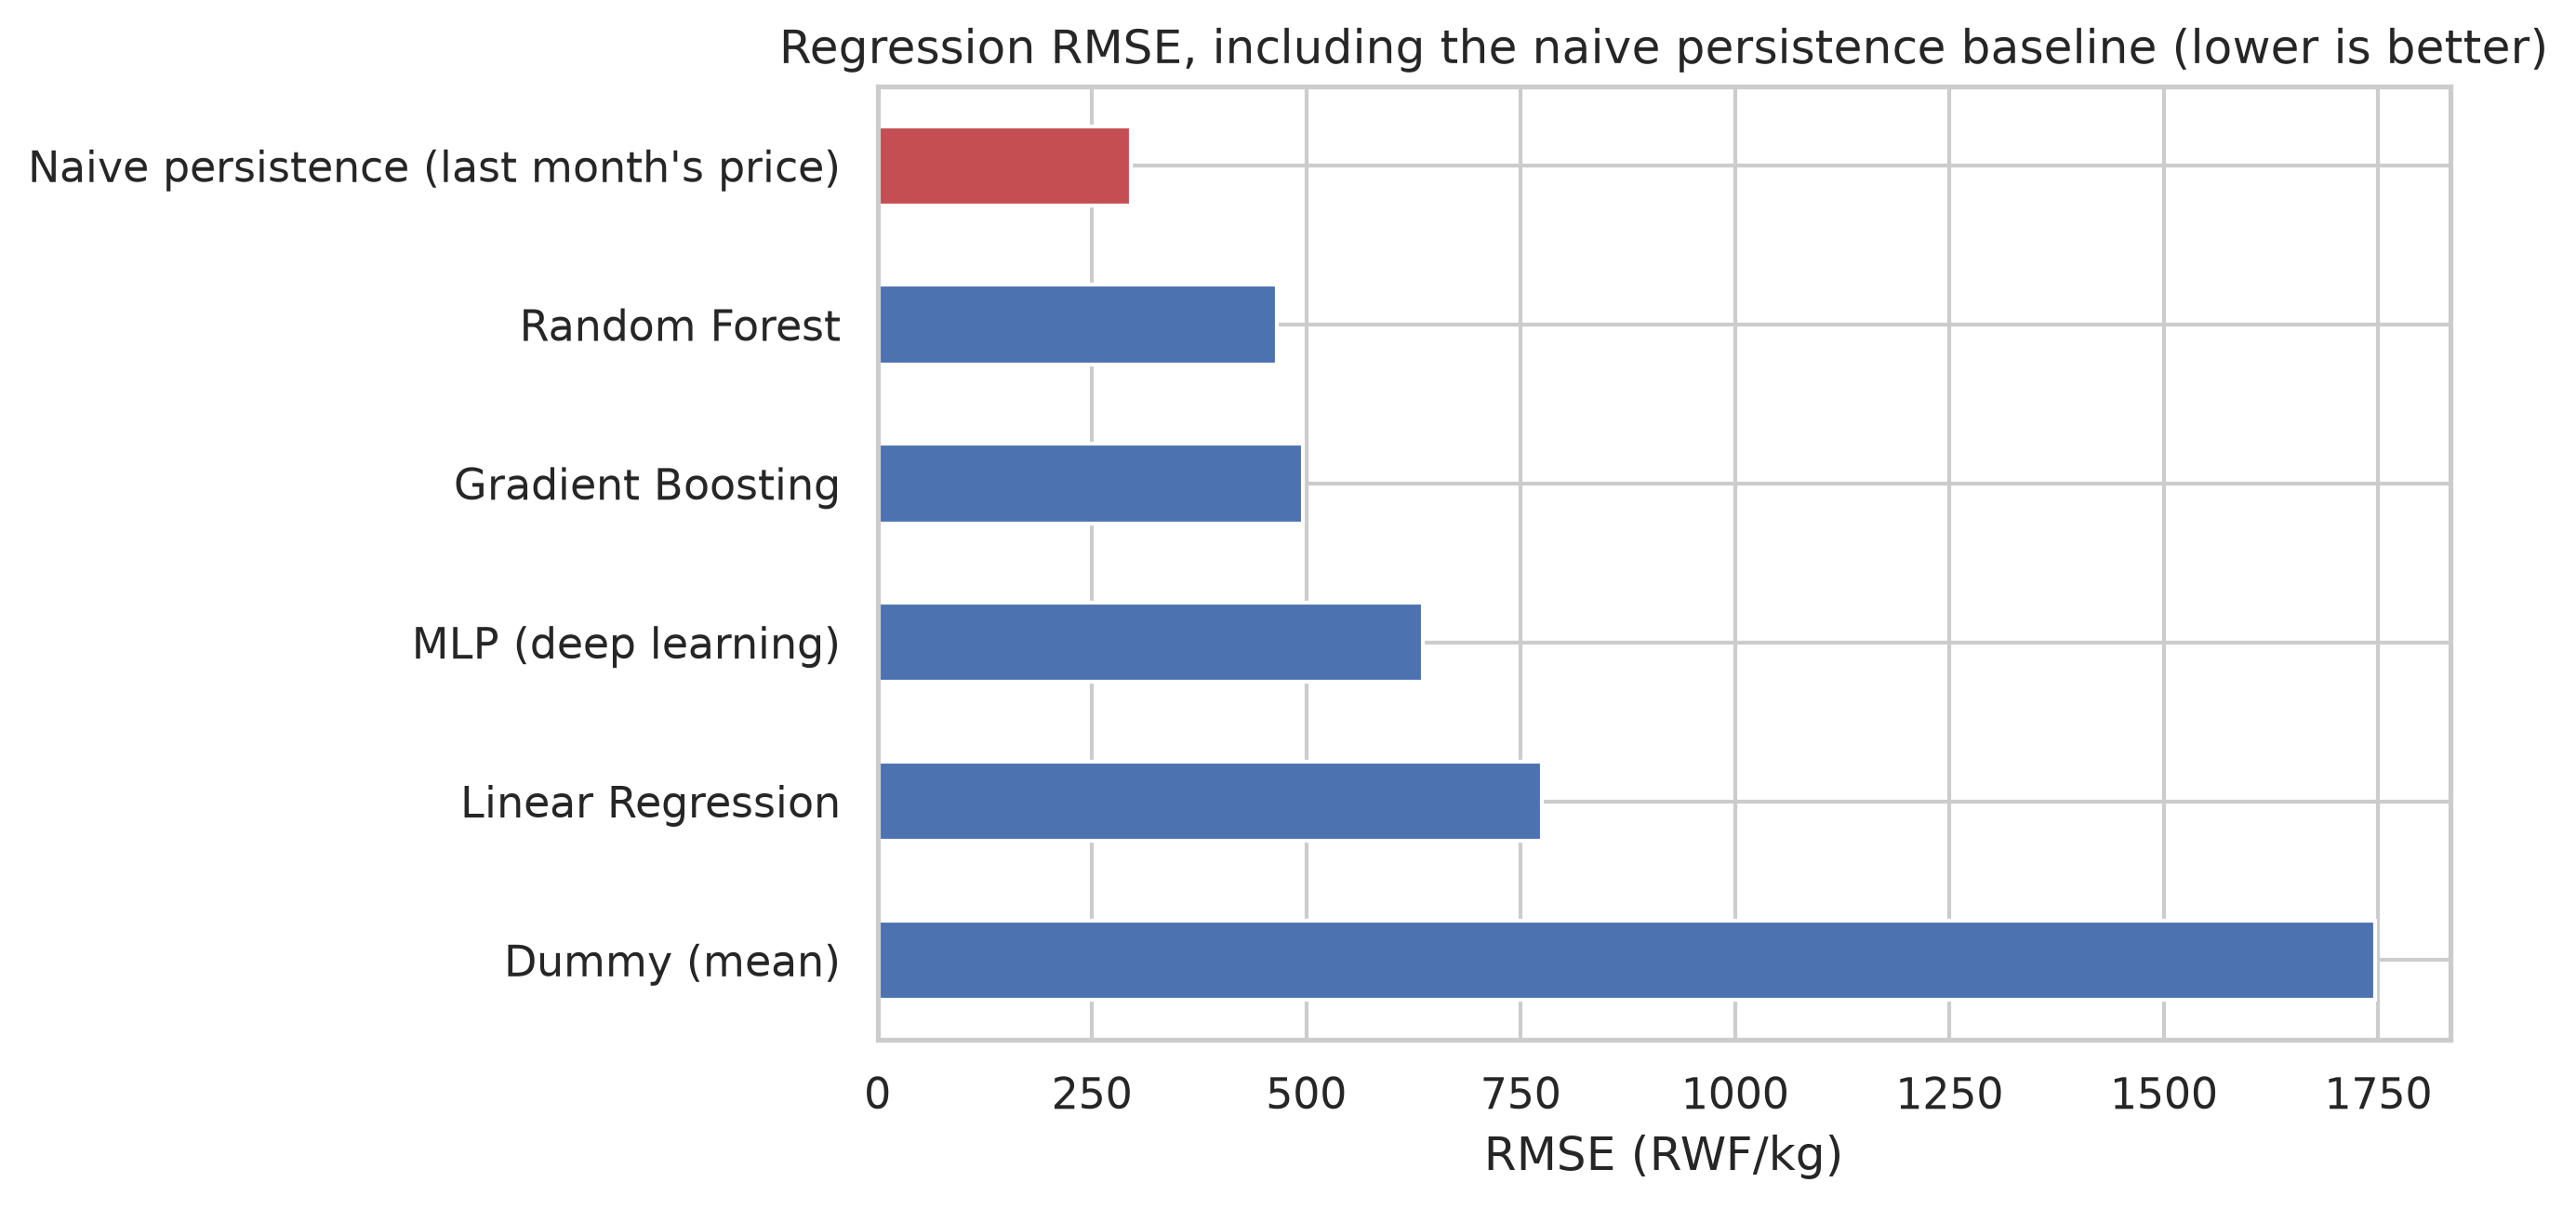
\includegraphics[width=0.85\textwidth]{regression_vs_persistence}
  \caption{Test-set RMSE including the naive persistence baseline (highlighted).
  No trained model improves on carrying the previous month's price forward.}
  \label{fig:persistence}
\end{figure}

\begin{figure}[H]
  \centering
  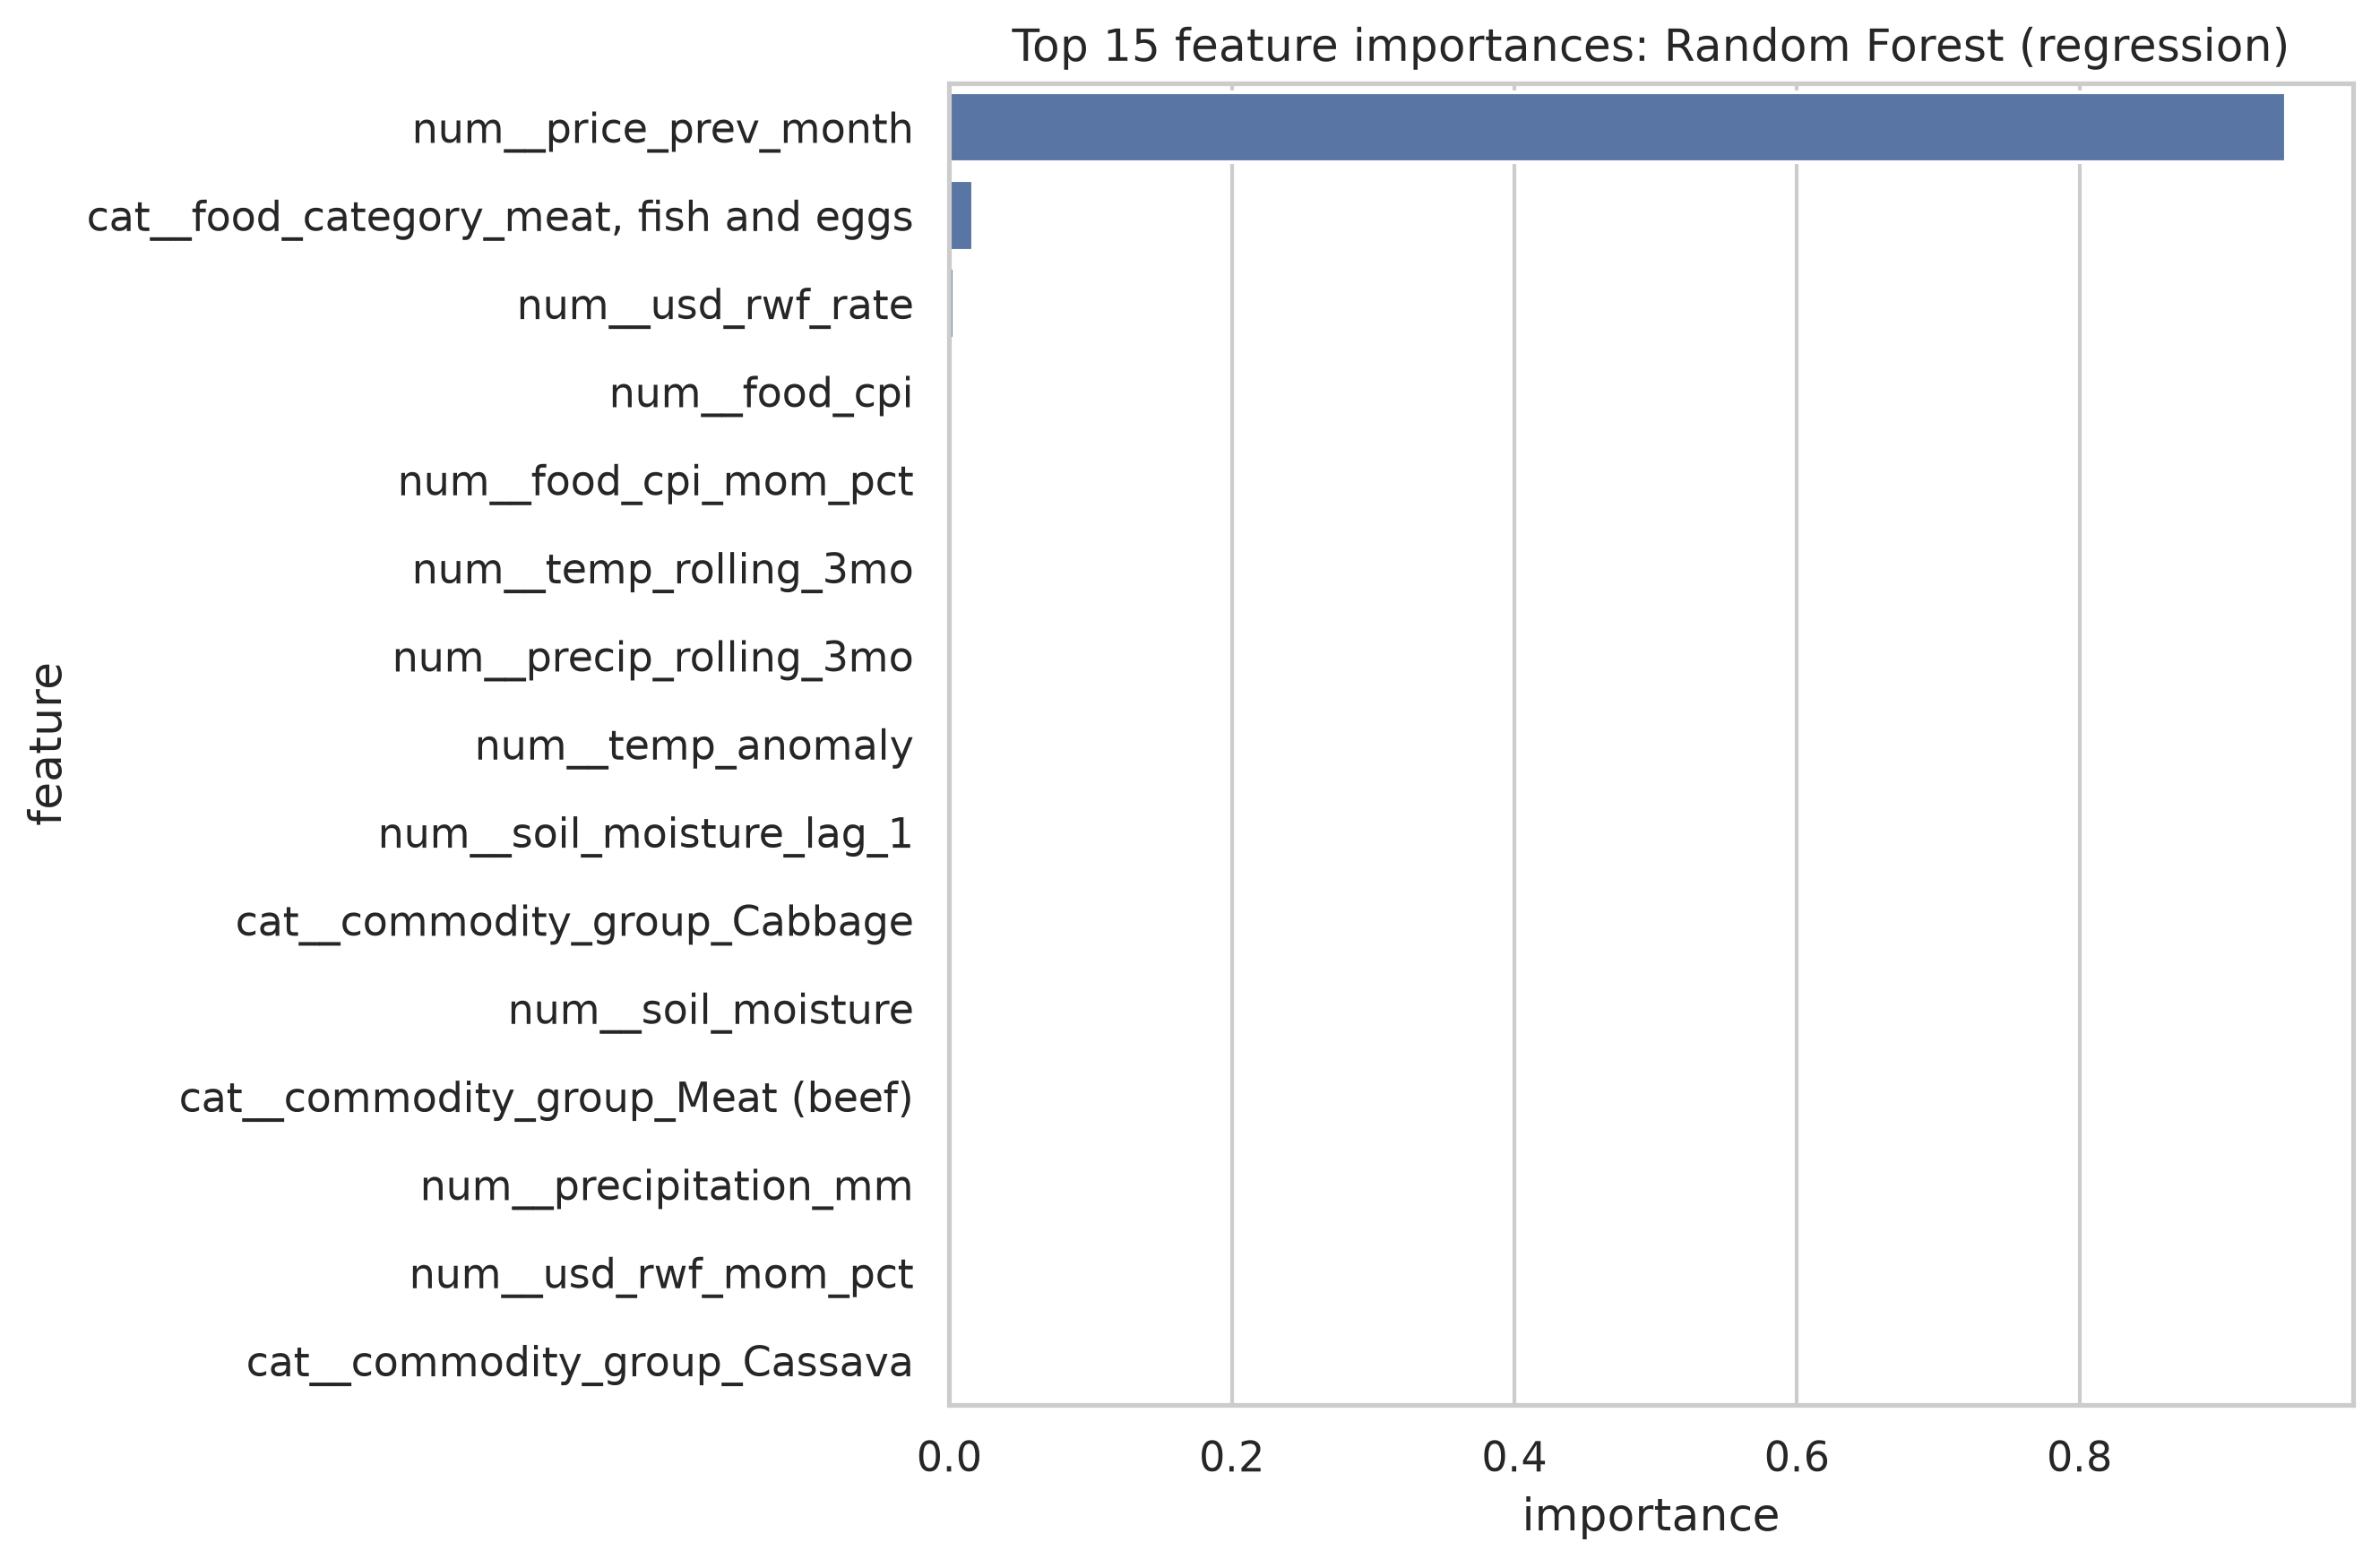
\includegraphics[width=0.85\textwidth]{feature_importance_regression}
  \caption{Top feature importances, random forest regressor.}
  \label{fig:importance}
\end{figure}

\subsection{Model Improvement}

With the corrected search space, tuning improved \emph{both} tasks  and, importantly, improved them on cross-validation before the test set was
consulted, so the gain is not an artifact of repeated test-set evaluation.

For classification the cross-validated F1 rose from 0.318 to 0.373 ($+0.055$), and the tuned model improved on the test set across accuracy
(0.607 to 0.628), precision (0.535 to 0.573), F1 (0.479 to 0.484), and ROC-AUC (0.608 to 0.641), at the cost of slightly lower recall
(Table~\ref{tab:tuning_clf}). For regression the cross-validated RMSE improved by 0.020 in log units, and test-set RMSE fell from 466 to 457 RWF with $R^2$
rising to 0.95 (Table~\ref{tab:tuning_reg}).

This is worth contrasting with the earlier, defective configuration described in Section~2.7, under which tuning appeared to \emph{degrade} regression
performance. The apparent degradation was an artifact of a search space that excluded the baseline's own hyperparameters; once corrected, tuning selected
\texttt{max\_depth=12} with \texttt{max\_features=0.5} and improved on the baseline as expected. The episode is a concrete illustration that a
counter-intuitive experimental result should prompt an audit of the experimental setup before it is written up as a finding about the data.

% AUTO-GENERATED by 3a_supervised_learning.ipynb -- do not edit by hand.
\begin{table}[H]
\centering
\caption{Classification: baseline vs.\ tuned (Random Forest).}
\label{tab:tuning_clf}
\begin{tabular}{lcc}
\toprule
 & Baseline & Tuned \\
\midrule
Accuracy & 0.607 & 0.628 \\
Precision & 0.535 & 0.573 \\
Recall & 0.434 & 0.418 \\
F1 & 0.479 & 0.484 \\
ROC-AUC & 0.608 & 0.641 \\
\bottomrule
\end{tabular}
\end{table}

% AUTO-GENERATED by 3a_supervised_learning.ipynb -- do not edit by hand.
\begin{table}[H]
\centering
\caption{Regression: baseline vs.\ tuned (Random Forest).}
\label{tab:tuning_reg}
\begin{tabular}{lcc}
\toprule
 & Baseline & Tuned \\
\midrule
RMSE (RWF) & 465.21 & 464.58 \\
MAE (RWF) & 192.08 & 195.12 \\
R2 (log scale) & 0.94 & 0.95 \\
\bottomrule
\end{tabular}
\end{table}


\subsection{Clustering: Market--Commodity Segmentation}

Silhouette analysis selects $k = \BestK{}$ (silhouette $= \Silhouette{}$ for K-Means, 0.539 for Ward linkage), indicating moderately well-separated
clusters. Algorithm agreement is informative in its own right (Table~\ref{tab:clustering_algos}): K-Means and Ward produce nearly identical
partitions (ARI $= \AriAgglo{}$), while the Gaussian mixture diverges substantially (ARI $= \AriGmm{}$, silhouette 0.320). This pattern is
interpretable rather than arbitrary. K-Means and Ward both favour compact, roughly spherical, equal-variance groups, whereas a Gaussian mixture fits
elliptical components with individual covariances. Their disagreement is therefore evidence about cluster \emph{shape}: the structure present here is
compact and spherical, which is the regime in which K-Means is the appropriate tool, and the two concordant algorithms are the ones whose assumptions match
the data.

The resulting clusters (Table~\ref{tab:clusters}) separate a small group of 26 market--commodity pairs  92.3\% of them in Northern Province  from the
remaining 323. The smaller cluster is cooler ($17.6^{\circ}$C versus $20.8^{\circ}$C), substantially wetter (4.72\,mm versus 3.34\,mm mean daily
precipitation, and 0.91 versus 0.74 soil moisture), roughly half as volatile in price (0.17 versus 0.31), and much less prone to month-over-month increases
(26\% versus 42\%).

Three observations follow. First, the clustering \emph{corroborates and sharpens} a pattern already visible in exploratory analysis rather than
discovering a new one: commodity composition is nearly identical across the two clusters, so the split reflects geography, not food type. Second,
precipitation and soil moisture separate the clusters at least as sharply as temperature does  Northern Province is not merely the coolest province but
also by a wide margin the wettest  which is direct evidence that the added climate variables carry information the temperature-only feature set did not.
Third, the smaller cluster's pairs rest on far fewer observations each (15.8 versus 39.4 on average), so its profile is a noisier estimate and every claim
about it is correspondingly weaker.

% AUTO-GENERATED by 3b_unsupervised_clustering.ipynb -- do not edit by hand.
\begin{table}[H]
\centering
\caption{Clustering algorithm comparison. ARI is measured against the K-Means partition (1.000 indicates an identical partition).}
\label{tab:clustering_algos}
\begin{tabular}{lcc}
\toprule
 & Silhouette Score & ARI vs. K-Means \\
Algorithm &  &  \\
\midrule
K-Means & 0.531 & 1.000 \\
Agglomerative (Ward) & 0.539 & 0.951 \\
Gaussian Mixture & 0.320 & 0.329 \\
\bottomrule
\end{tabular}
\end{table}

% AUTO-GENERATED by 3b_unsupervised_clustering.ipynb -- do not edit by hand.
\begin{table}[H]
\centering
\caption{K-Means cluster profiles (k=2, silhouette=0.531).}
\label{tab:clusters}
\begin{tabular}{lcccccccc}
\toprule
 & avg\_log\_price & price\_volatility & avg\_temp & avg\_precip & avg\_soil\_moisture & pct\_price\_increase & n\_observations & n\_pairs \\
cluster &  &  &  &  &  &  &  &  \\
\midrule
0 & 6.50 & 0.31 & 20.83 & 3.34 & 0.74 & 0.42 & 39.36 & 323 \\
1 & 6.12 & 0.17 & 17.63 & 4.72 & 0.91 & 0.26 & 15.77 & 26 \\
\bottomrule
\end{tabular}
\end{table}


\begin{figure}[H]
  \centering
  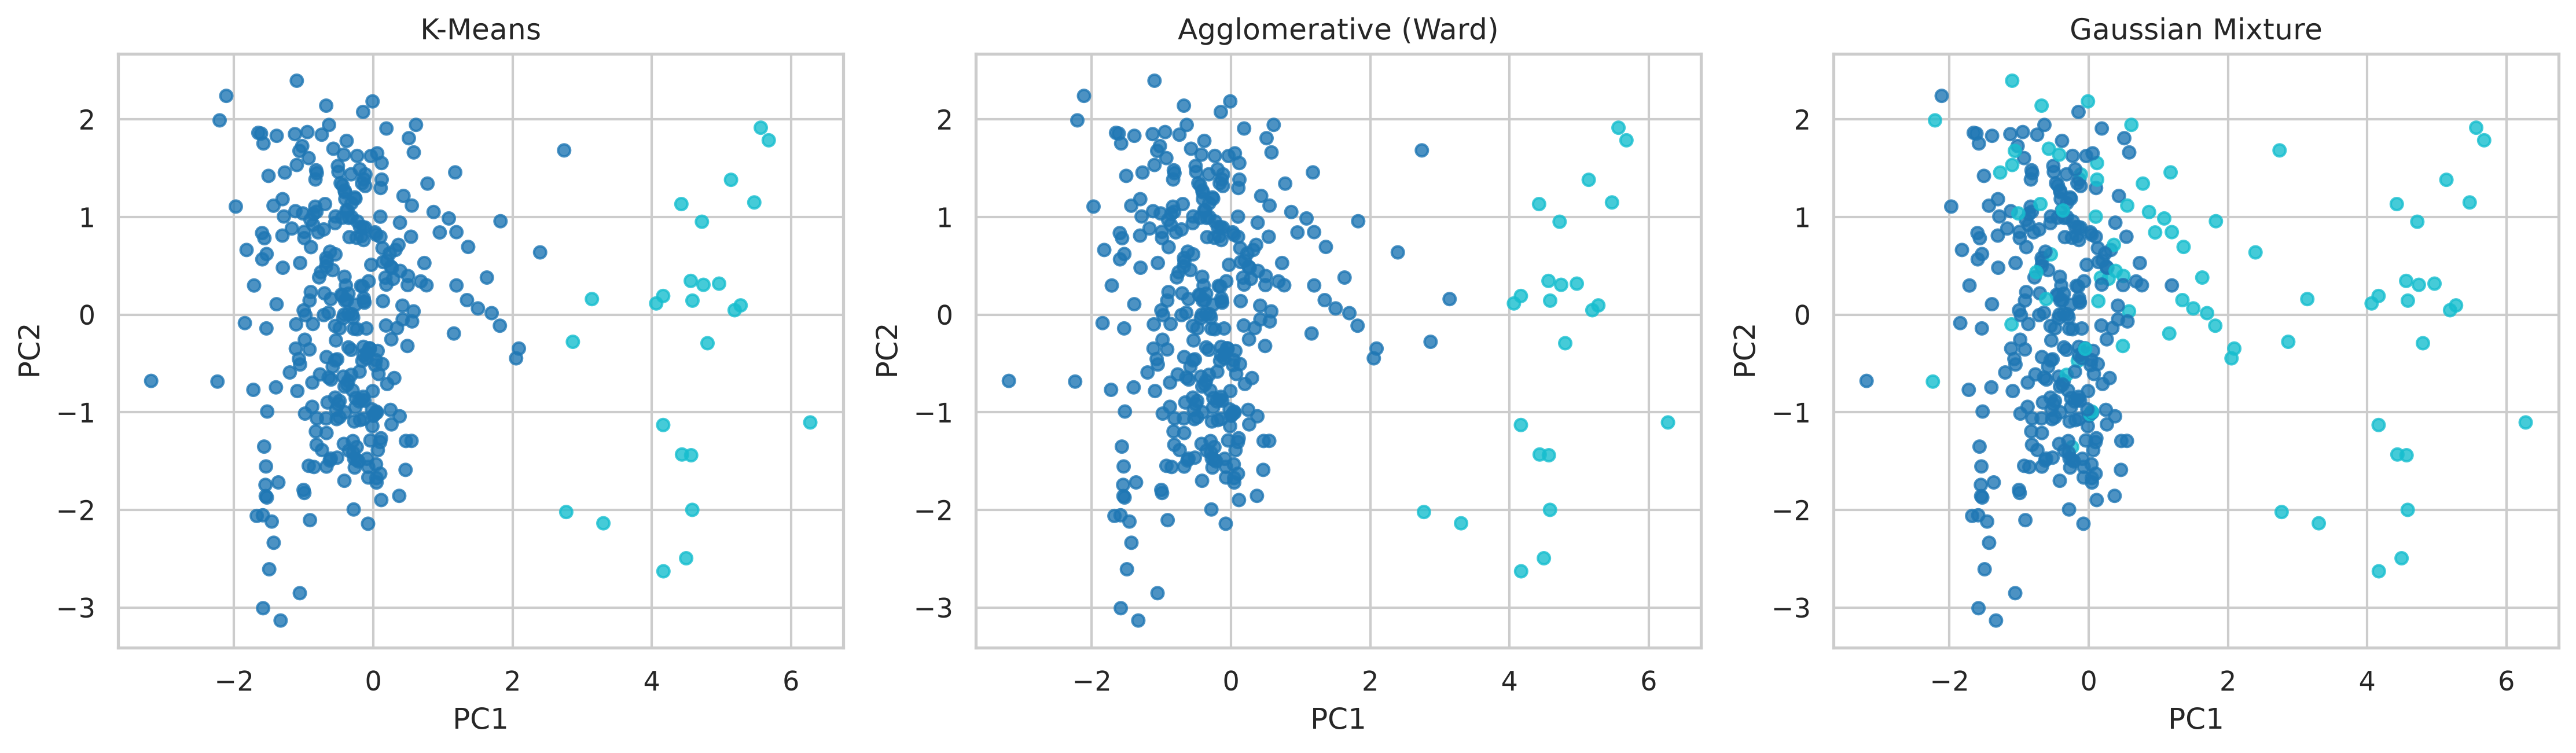
\includegraphics[width=\textwidth]{cluster_comparison_pca}
  \caption{PCA projection of clustering results for all three algorithms.}
  \label{fig:cluster_pca}
\end{figure}

\begin{figure}[H]
  \centering
  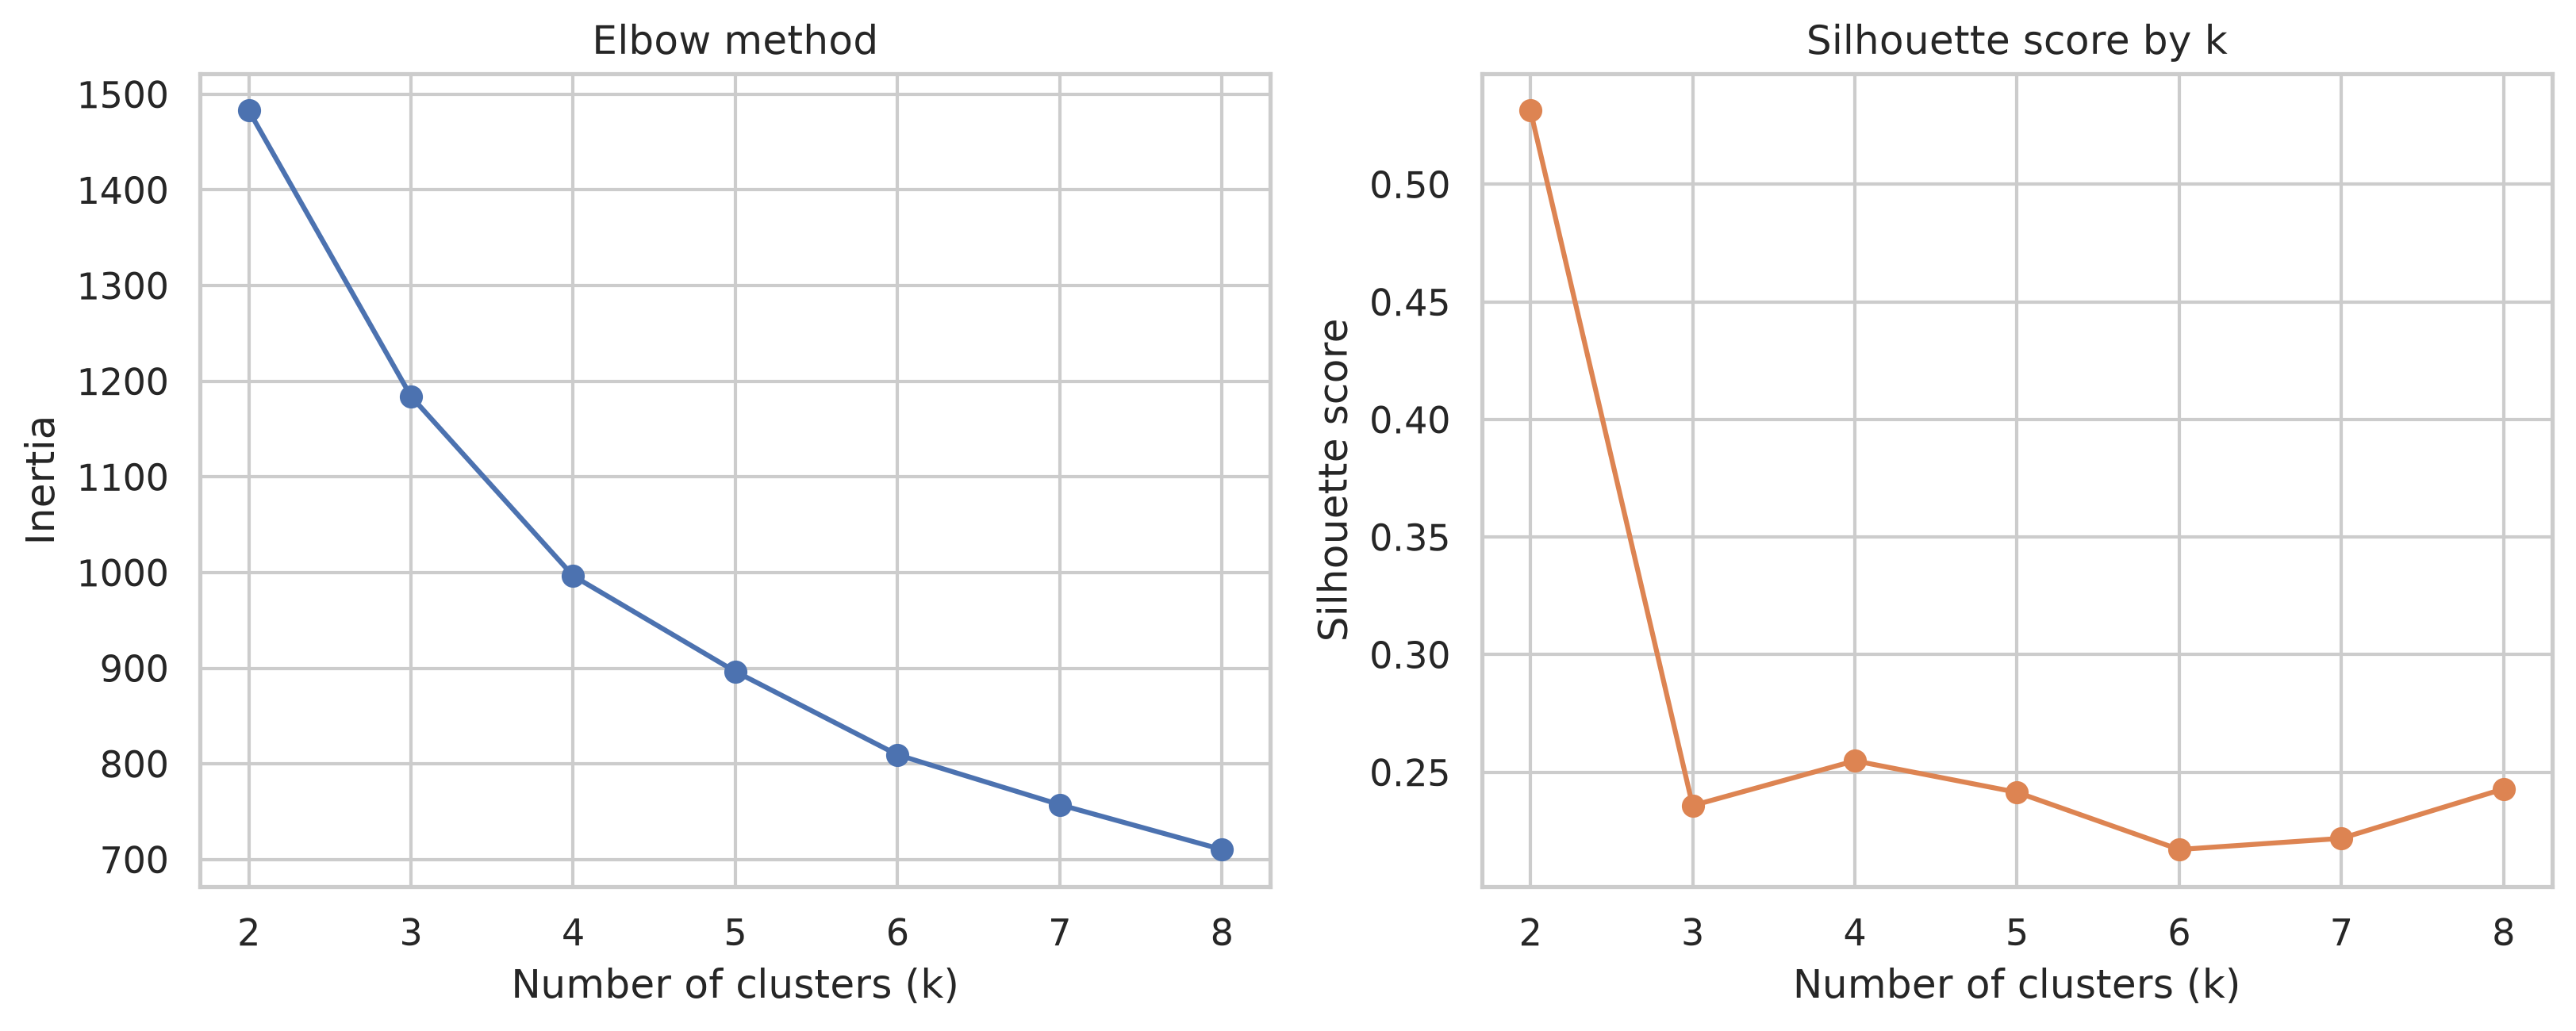
\includegraphics[width=0.85\textwidth]{cluster_k_selection}
  \caption{Elbow method and silhouette score across candidate $k$.}
  \label{fig:cluster_k}
\end{figure}

\section{Discussion and Recommendations}
\label{sec:discussion}

\subsection{Price Level and Price Direction Are Different Problems}

The apparent gap between regression ($R^2 = 0.94$) and classification (ROC-AUC 0.641) initially suggests that price levels are easy to predict and directions
hard. The persistence benchmark shows the first half of that statement needs qualification.

Price \emph{level} is dominated by two quantities that require no modelling: which commodity it is, and what it cost last month. Together these account for
essentially all of the achievable fit, and a zero-parameter persistence rule outperforms every algorithm compared here. The regression task is therefore
not so much \emph{solved} as \emph{trivial}  there is little structure left for a model to exploit once autocorrelation is accounted for, and the flexible
learners add variance without adding signal.

Price \emph{direction} admits no such trivial rule: knowing last month's price tells you nothing about the sign of next month's change. That task depends on
month-to-month \emph{changes} driven by supply shocks, harvest timing, and transport costs the dataset does not observe, and it is there  against a
majority-class baseline that no shortcut can beat  that the trained models demonstrably add value, if modestly.

The practical implication is sharper than the raw metrics suggest. A food security system that reports impressive $R^2$ on price levels may be doing
nothing more than echoing last month's prices back to its users, while the directional question that actually matters for early warning remains the hard
one. The two capabilities should not be conflated, and a level-prediction model should always be reported against a persistence benchmark rather than a mean
baseline.

\subsection{The Enrichment Helped, but Not for the Hypothesised Reason}
\label{sec:ablation}

Because the enriched and temperature-only pipelines were run over \emph{identical} rows (\NRows{}) with an \emph{identical} chronological split
(\NTrain{} training, \NTest{} test), the comparison between them is a controlled ablation in which only the feature set differs.

Under that comparison, ROC-AUC improved for every model family: logistic regression from 0.586 to 0.588, random forest from 0.556 to 0.608, gradient
boosting from 0.572 to 0.610, and the MLP from 0.591 to 0.610, with the tuned random forest reaching 0.641. Regression RMSE improved from 480 to 466 RWF,
and to 457 after tuning.

One metric moved the other way and should not be glossed over: the best F1 fell from 0.552 to 0.479. That earlier figure came from a logistic regression with
recall of 0.697  a model that predicted ``increase'' aggressively and was rewarded for it at the default 0.5 threshold. The enriched models are more
conservative and better \emph{ranked}. Since ROC-AUC measures threshold-independent discrimination while F1 measures performance at one
arbitrary threshold, the consistent ROC-AUC gain is the more reliable evidence that the enrichment improved the models; a practitioner wanting higher recall
would tune the decision threshold rather than revert the feature set.

The more interesting result concerns \emph{which} features earned the gain. The hypothesis motivating this data collection was that \emph{macroeconomic}
pressure  exchange rate depreciation and inflation  would explain directional movement that weather could not. The evidence does not support
that attribution. In the direction-split analysis, precipitation separates rising from falling observations by roughly 0.33\,mm per day (3.01 versus
3.33), while month-over-month food CPI, general CPI, and exchange rate changes differ between the classes by 0.006, 0.003, and 0.0005 respectively. The
clustering result points the same way, with precipitation and soil moisture emerging as primary discriminators alongside temperature.

The most defensible reading is that the improvement came chiefly from measuring \emph{climate} better  moving from air temperature alone to
variables closer to actual growing conditions  rather than from adding national macroeconomic context. A plausible mechanism is that the
macroeconomic series vary only by date and are therefore constant across all markets in a given month, so they can shift the overall price trend but cannot
explain why one market's maize rose while another's fell; precipitation, which varies by province, can. We report this because it is what the data shows
rather than what the data collection was designed to demonstrate.

\subsection{Limitations}

\begin{itemize}
  \item \textbf{Uneven geographic coverage.} Kigali City and Northern Provinceare substantially under-represented relative to Eastern and Southern
        Provinces. This bears directly on the clustering result: the Northern Province cluster comprises 22 pairs averaging roughly 10
        observations each, against about 35 for the larger cluster, so its profile is a noisier estimate and claims about it are correspondingly
        weaker.
  \item \textbf{An unverified CPI publication-lag assumption.} The one-month lag is a conservative default, not a confirmed feature of NISR's
        release calendar. If the true lag differs, the CPI features' apparent contribution should be re-assessed under corrected alignment.
  \item \textbf{A disclosed climatological simplification.} Monthly baselines for \texttt{temp\_anomaly} and \texttt{precip\_anomaly} are averaged
        over the full 2020--2026 span rather than an expanding window, so an early observation's ``seasonal normal'' is partly informed by later
        years. This mirrors standard meteorological practice for climate normals but is technically mild look-ahead information.
  \item \textbf{Constrained hyperparameter search.} The search budget was limited by available compute. The corrected grids contain each
        baseline configuration, but a wider search may still find configurations this one did not reach.
  \item \textbf{Limited headroom on the regression task.} Because a naive persistence forecast outperforms every trained model, the level-prediction
        results should not be read as evidence of forecasting skill. A more informative formulation would target the \emph{change} in price directly
        (i.e.\ model $p_t - p_{t-1}$ rather than $p_t$), which removes the autocorrelation that dominates the current target.
  \item \textbf{Aggregate rather than commodity-specific modelling.} A single model is fitted across all commodity groups, despite exploratory
        evidence that climate sensitivity differs sharply between fresh produce and processed staples.
\end{itemize}

\subsection{Recommendations}

Four directions follow from these results. First, and most directly implied by Section~\ref{sec:discussion}, effort is better spent on further
\emph{agronomic} measurement  crop calendars, growing-degree days, commodity-specific planting and harvest windows  than on additional
national macroeconomic aggregates, since the former is where the observed improvement originated. Second, fitting separate models per commodity group,
or adding explicit commodity--climate interaction terms, would test the exploratory finding that weather-sensitive and processed commodities respond
differently. Third, NISR's actual CPI release calendar should be verified so the publication-lag assumption can be replaced with a fact. Fourth, extending
the pipeline to Kenya, Tanzania, and Uganda would increase sample size for under-represented categories and test whether the Northern Province pattern
generalises to comparable highland regions elsewhere in East Africa.

\bibliographystyle{apalike}
\bibliography{references}

\end{document}
